% Options for packages loaded elsewhere
\PassOptionsToPackage{unicode}{hyperref}
\PassOptionsToPackage{hyphens}{url}
%
\documentclass[
  12pt,
]{article}
\usepackage{amsmath,amssymb}
\usepackage{iftex}
\ifPDFTeX
  \usepackage[T1]{fontenc}
  \usepackage[utf8]{inputenc}
  \usepackage{textcomp} % provide euro and other symbols
\else % if luatex or xetex
  \usepackage{unicode-math} % this also loads fontspec
  \defaultfontfeatures{Scale=MatchLowercase}
  \defaultfontfeatures[\rmfamily]{Ligatures=TeX,Scale=1}
\fi
\usepackage{lmodern}
\ifPDFTeX\else
  % xetex/luatex font selection
\fi
% Use upquote if available, for straight quotes in verbatim environments
\IfFileExists{upquote.sty}{\usepackage{upquote}}{}
\IfFileExists{microtype.sty}{% use microtype if available
  \usepackage[]{microtype}
  \UseMicrotypeSet[protrusion]{basicmath} % disable protrusion for tt fonts
}{}
\makeatletter
\@ifundefined{KOMAClassName}{% if non-KOMA class
  \IfFileExists{parskip.sty}{%
    \usepackage{parskip}
  }{% else
    \setlength{\parindent}{0pt}
    \setlength{\parskip}{6pt plus 2pt minus 1pt}}
}{% if KOMA class
  \KOMAoptions{parskip=half}}
\makeatother
\usepackage{xcolor}
\usepackage{color}
\usepackage{fancyvrb}
\newcommand{\VerbBar}{|}
\newcommand{\VERB}{\Verb[commandchars=\\\{\}]}
\DefineVerbatimEnvironment{Highlighting}{Verbatim}{commandchars=\\\{\}}
% Add ',fontsize=\small' for more characters per line
\usepackage{framed}
\definecolor{shadecolor}{RGB}{248,248,248}
\newenvironment{Shaded}{\begin{snugshade}}{\end{snugshade}}
\newcommand{\AlertTok}[1]{\textcolor[rgb]{0.94,0.16,0.16}{#1}}
\newcommand{\AnnotationTok}[1]{\textcolor[rgb]{0.56,0.35,0.01}{\textbf{\textit{#1}}}}
\newcommand{\AttributeTok}[1]{\textcolor[rgb]{0.13,0.29,0.53}{#1}}
\newcommand{\BaseNTok}[1]{\textcolor[rgb]{0.00,0.00,0.81}{#1}}
\newcommand{\BuiltInTok}[1]{#1}
\newcommand{\CharTok}[1]{\textcolor[rgb]{0.31,0.60,0.02}{#1}}
\newcommand{\CommentTok}[1]{\textcolor[rgb]{0.56,0.35,0.01}{\textit{#1}}}
\newcommand{\CommentVarTok}[1]{\textcolor[rgb]{0.56,0.35,0.01}{\textbf{\textit{#1}}}}
\newcommand{\ConstantTok}[1]{\textcolor[rgb]{0.56,0.35,0.01}{#1}}
\newcommand{\ControlFlowTok}[1]{\textcolor[rgb]{0.13,0.29,0.53}{\textbf{#1}}}
\newcommand{\DataTypeTok}[1]{\textcolor[rgb]{0.13,0.29,0.53}{#1}}
\newcommand{\DecValTok}[1]{\textcolor[rgb]{0.00,0.00,0.81}{#1}}
\newcommand{\DocumentationTok}[1]{\textcolor[rgb]{0.56,0.35,0.01}{\textbf{\textit{#1}}}}
\newcommand{\ErrorTok}[1]{\textcolor[rgb]{0.64,0.00,0.00}{\textbf{#1}}}
\newcommand{\ExtensionTok}[1]{#1}
\newcommand{\FloatTok}[1]{\textcolor[rgb]{0.00,0.00,0.81}{#1}}
\newcommand{\FunctionTok}[1]{\textcolor[rgb]{0.13,0.29,0.53}{\textbf{#1}}}
\newcommand{\ImportTok}[1]{#1}
\newcommand{\InformationTok}[1]{\textcolor[rgb]{0.56,0.35,0.01}{\textbf{\textit{#1}}}}
\newcommand{\KeywordTok}[1]{\textcolor[rgb]{0.13,0.29,0.53}{\textbf{#1}}}
\newcommand{\NormalTok}[1]{#1}
\newcommand{\OperatorTok}[1]{\textcolor[rgb]{0.81,0.36,0.00}{\textbf{#1}}}
\newcommand{\OtherTok}[1]{\textcolor[rgb]{0.56,0.35,0.01}{#1}}
\newcommand{\PreprocessorTok}[1]{\textcolor[rgb]{0.56,0.35,0.01}{\textit{#1}}}
\newcommand{\RegionMarkerTok}[1]{#1}
\newcommand{\SpecialCharTok}[1]{\textcolor[rgb]{0.81,0.36,0.00}{\textbf{#1}}}
\newcommand{\SpecialStringTok}[1]{\textcolor[rgb]{0.31,0.60,0.02}{#1}}
\newcommand{\StringTok}[1]{\textcolor[rgb]{0.31,0.60,0.02}{#1}}
\newcommand{\VariableTok}[1]{\textcolor[rgb]{0.00,0.00,0.00}{#1}}
\newcommand{\VerbatimStringTok}[1]{\textcolor[rgb]{0.31,0.60,0.02}{#1}}
\newcommand{\WarningTok}[1]{\textcolor[rgb]{0.56,0.35,0.01}{\textbf{\textit{#1}}}}
\usepackage{longtable,booktabs,array}
\usepackage{calc} % for calculating minipage widths
% Correct order of tables after \paragraph or \subparagraph
\usepackage{etoolbox}
\makeatletter
\patchcmd\longtable{\par}{\if@noskipsec\mbox{}\fi\par}{}{}
\makeatother
% Allow footnotes in longtable head/foot
\IfFileExists{footnotehyper.sty}{\usepackage{footnotehyper}}{\usepackage{footnote}}
\makesavenoteenv{longtable}
\usepackage{graphicx}
\makeatletter
\def\maxwidth{\ifdim\Gin@nat@width>\linewidth\linewidth\else\Gin@nat@width\fi}
\def\maxheight{\ifdim\Gin@nat@height>\textheight\textheight\else\Gin@nat@height\fi}
\makeatother
% Scale images if necessary, so that they will not overflow the page
% margins by default, and it is still possible to overwrite the defaults
% using explicit options in \includegraphics[width, height, ...]{}
\setkeys{Gin}{width=\maxwidth,height=\maxheight,keepaspectratio}
% Set default figure placement to htbp
\makeatletter
\def\fps@figure{htbp}
\makeatother
\setlength{\emergencystretch}{3em} % prevent overfull lines
\providecommand{\tightlist}{%
  \setlength{\itemsep}{0pt}\setlength{\parskip}{0pt}}
\setcounter{secnumdepth}{5}
\usepackage[a4paper, top=2.5cm, bottom=2.5cm, left=2.5cm, right=2.5cm]{geometry} \usepackage{pdfpages} \usepackage{framed} \usepackage{mathptmx} \usepackage[french,]{babel} \usepackage[utf8]{inputenc} \usepackage[T1]{fontenc} \usepackage[table, xcdraw, dvipsnames]{xcolor} \usepackage{graphicx} \usepackage{hyperref} \usepackage{tikz} \usepackage{fancyhdr} % For heading and footers, les entêtes et les pieds de pages
%\frenchbsetup{StandardLists=true} % à inclure si on utilise
%\usepackage[french]{babel} \usepackage{enumitem} % pour les items numérotés
%\usepackage[Lenny]{fncychap} \usepackage{multicol} % Pour diviser la page, la moitié
%\usepackage{pdfpages} % Pour importer des pdf
%\usepackage{multirow}
%\usepackage{array} % environnement nécessaire pour les maths
\usepackage{amsmath,amssymb} % environnement nécessaire pour les maths
\usepackage{iftex} \usepackage{textcomp} \usepackage[]{microtype} \usepackage{longtable,booktabs,array} % necessaire pour les longs tableaux
\usepackage{calc} \usepackage[Conny]{fncychap} \usepackage{setspace} % pour l'espacement, l'interligne
\usepackage{MnSymbol} \definecolor{gre}{RGB}{101, 191, 127} \definecolor{gree}{RGB}{7, 135, 44} \usepackage[most, many]{tcolorbox} \geometry{hmargin  = 2.5cm, vmargin = 1.5cm} % pour régler les marges
\renewcommand\thesection{\Roman{section}}
\usepackage{booktabs}
\usepackage{longtable}
\usepackage{array}
\usepackage{multirow}
\usepackage{wrapfig}
\usepackage{float}
\usepackage{colortbl}
\usepackage{pdflscape}
\usepackage{tabu}
\usepackage{threeparttable}
\usepackage{threeparttablex}
\usepackage[normalem]{ulem}
\usepackage{makecell}
\usepackage{xcolor}
\ifLuaTeX
  \usepackage{selnolig}  % disable illegal ligatures
\fi
\usepackage{bookmark}
\IfFileExists{xurl.sty}{\usepackage{xurl}}{} % add URL line breaks if available
\urlstyle{same}
\hypersetup{
  hidelinks,
  pdfcreator={LaTeX via pandoc}}

\author{}
\date{\vspace{-2.5em}}

\begin{document}


\includepdf{Page de garde 3.pdf}


\includepdf{Photo2.pdf}

\begin{center}
\includegraphics[width=1\linewidth,height=1\textheight]{../Document_Rmarkdown/R} \end{center}

\newpage

\textcolor{blue}{\tableofcontents}

\newpage

\listoftables
\listoffigures
\newpage

\renewcommand{\headrulewidth}{1.5pt}
\let\oldheadrule\headrule                            
\renewcommand{\headrule}{\color{blue}\oldheadrule}% Add colour to \headrule
\renewcommand{\footrulewidth}{1.5pt} 
\let\oldfootrule\footrule%
\renewcommand{\footrule}{\color{blue}\oldfootrule}% Add colour to \headrule
\pagestyle{fancy}        %Default page style 
\lhead{\scriptsize{R-Markdown}} % left head entête gauche
\chead{} % entête Au centre
\rhead{\textcolor{black}{2024}} % right head entête à droite
\lfoot{\textcolor{black}{ENSAE}} % pieds de page gauche 
\rfoot{Groupe 5} % Au centre du pied de page 
%
%\section*{{Introduction}\addcontentsline{toc}{section}{Introduction}} 
% l'etoile '*' permet de ne pas compter une section comme un titre

\section{Introduction}\label{introduction}

La création d'un rapport, d'un mémoire ou même d'une thèse à caractère
scientifique nécessite très souvent d'y faire apparaître des tableaux,
des graphiques voire même des lignes de codes explicites. Les logiciels
classiques tels que Ms Word et LateX requièrent des procédés ambiguës
pour insérer de tels éléments. R Markdown est un outil qui réponds à de
telles préoccupations.

\subsection{C'est quoi au fait R Markdown
?}\label{cest-quoi-au-fait-r-markdown}

Avant de definir R markdown, nous allons au préalable definir le langage
Markdown. Le langage Markdown est un langage de balisage léger qui
permet de formater du texte de manière simple et lisible, en utilisant
des caractères typographiques courants. R Markdown est une variante de
markdown qui est spécifique à R. Il permet d'écrire un document en
utilisant markdown pour produire du texte et pour incorporer du code R,
Python, SQL et bien d'autres et afficher leurs sorties. Les fichiers R
Markdown ont une extension \texttt{.Rmd}.

\subsection{Pourquoi R Markdown est-il aussi important
?}\label{pourquoi-r-markdown-est-il-aussi-important}

R Markdown est un outil très important. En effet, R Markdown offre une
grande flexibilité et diversité en termes de formats de sortie pour les
documents. Il permet les formats de sortie suivant :

\begin{itemize}
\item
  \textbf{HTML} : Les documents HTML peuvent être interactifs et inclure
  des éléments comme des graphiques interactifs (avec des bibliothèques
  comme Plotly), des tableaux de données dynamiques (avec DataTables),
  etc.
\item
  \textbf{PDF}
\item
  \textbf{Word}
\item
  \textbf{Présentations} : R Markdown prend en charge la création de
  présentations au format HTML ou PDF.
\item
  \textbf{Dashboards interactifs} : Avec des packages comme
  flexdashboard ou shiny, on peut créer des tableaux de bord interactifs
  à partir de R Markdown. Ces tableaux de bord peuvent inclure des
  graphiques interactifs, des widgets de contrôle, etc.
\item
  \textbf{Livres électroniques (e-books)} : On peut générer des livres
  électroniques au format EPUB ou Kindle à partir de R Markdown. Cela
  peut être utile si vous écrivez un livre ou un document plus long et
  que vous souhaitez le distribuer sous forme de livre électronique.
\item
  \textbf{Beamer (pour les présentations LaTeX)}
\end{itemize}

D'autre part, R Markdown est un outil puissant qui permet de combiner du
code R, des résultats de code, et du texte formaté dans un document
unique. Voici quelques-unes de ses principales fonctionnalités :

\begin{itemize}
\item
  \textbf{Intégration de code} : Vous pouvez intégrer du code R
  directement dans votre document Markdown en utilisant des blocs de
  code délimités par trois backticks (```). Ce code peut être exécuté
  lors de la génération du document, et les résultats peuvent être
  affichés directement dans le document.
\item
  \textbf{Rendu dynamique} : R Markdown permet de générer une grande
  variété de formats de sortie, y compris HTML, PDF, Word, présentations
  (via HTML ou PDF), et bien d'autres. Vous pouvez spécifier le format
  de sortie dans les métadonnées du document ou lors de la génération du
  document.
\item
  \textbf{Mixage de formats de texte} : Vous pouvez utiliser du texte
  formaté en Markdown pour structurer votre document (titres, listes,
  etc.), ainsi que du texte en LaTeX pour des formattages plus avancés
  (équations mathématiques, références bibliographiques, etc.).
\item
  \textbf{Incorporation de graphiques} : R Markdown permet de générer et
  d'inclure des graphiques générés par R (à l'aide de ggplot2, base R,
  etc.) directement dans le document final. Les graphiques sont
  automatiquement insérés à l'endroit où vous spécifiez le code pour les
  créer.
\item
  \textbf{Support de nombreux langages de programmation} : Bien que son
  nom suggère une utilisation principale avec R, R Markdown prend en
  charge d'autres langages de programmation comme Python, Julia, et bien
  d'autres. Vous pouvez intégrer et exécuter du code dans ces langages
  dans le même document.
\item
  \textbf{Personnalisation avancée} : Vous pouvez personnaliser de
  nombreux aspects de votre document final, y compris le style, les
  polices, les marges, etc., en utilisant des options spécifiques au
  format de sortie ou en passant par des fichiers de configuration.
\item
  \textbf{Facilité d'utilisation} : R Markdown est conçu pour être
  convivial, même pour les débutants. Sa syntaxe est relativement simple
  et intuitive, ce qui en fait un choix populaire pour la génération de
  rapports, de documents de recherche, de présentations, etc.
\end{itemize}

Tout autre détail sur le langage R Markdown peut être obtenu à partir du
lien suivant: \url{http://rmarkdown.rstudio.com}.

\newpage

\section{Utilisation de R markdown}\label{utilisation-de-r-markdown}

\subsection{Installation du package de R
markdown}\label{installation-du-package-de-r-markdown}

Pour installer le package R Markdown, on peut utiliser directement la
fonction \texttt{install.packages()}:
\texttt{install.packages("rmarkdown")}

Pour charger le package R Markdown, on utilise la fonction
\texttt{library()} : \texttt{library(rmarkdown)}

On peut aussi aller dans la fenêtre de presentation et puis cliquer sur
\texttt{packages} ensuite install et enfin selectionner l'installation à
partir du CRAN, entrer le nom du package Rmarkdown et cliquer sur
\texttt{Installer}.

\begin{center}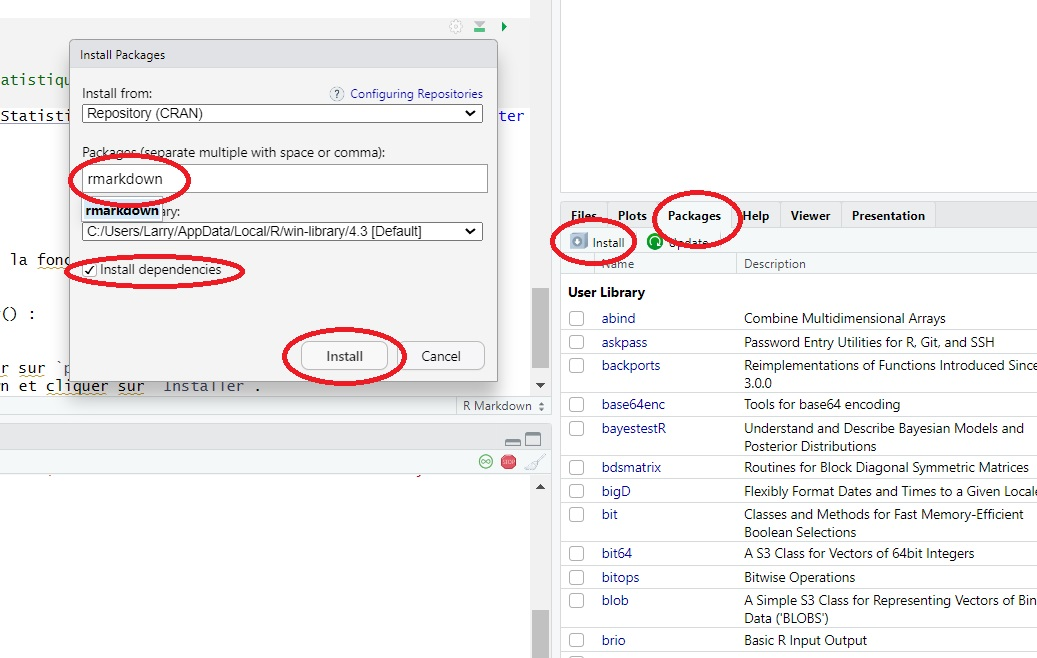
\includegraphics[width=0.6\linewidth,height=0.6\textheight]{../Document_Rmarkdown/Images/Installation_package_Rmd} \end{center}

\textbf{\emph{NB :}} Toujours prendre la peine de cocher sur
\texttt{install\ dependencies}.

\subsection{Présentation de l'environnement R
Markdown}\label{pruxe9sentation-de-lenvironnement-r-markdown}

Dans cette partie, nous allons vous présenter les bases de R markdown.

\subsubsection{Structure d'un document R
Markdown}\label{structure-dun-document-r-markdown}

Lorsque votre logiciel RStudio est ouvert, pour ouvrir un fichier R
markdown, vous pouvez cliquer sur \texttt{new\ file} et ensuite choisir
le fichier \texttt{R\ markdown}.

Comme cela est illustré sur la photo ci-dessous:

\begin{center}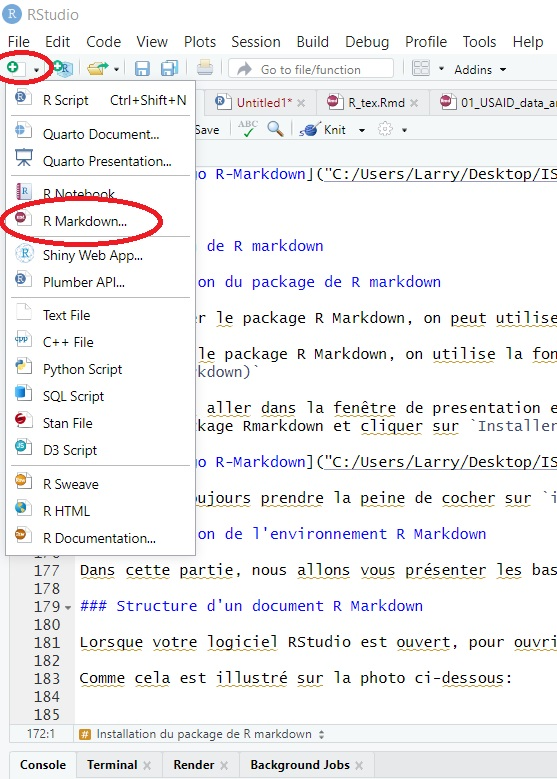
\includegraphics[width=0.6\linewidth,height=0.4\textheight]{../Document_Rmarkdown/Images/Creation_fichier_Rmd} \end{center}

La fenêtre ci-dessous s'ouvre alors sur laquelle vous pouvez spécifier
le titre de votre document, le nom de l'auteur, la date et le format de
sortie ( HTML, pdf ou Word) :

\begin{center}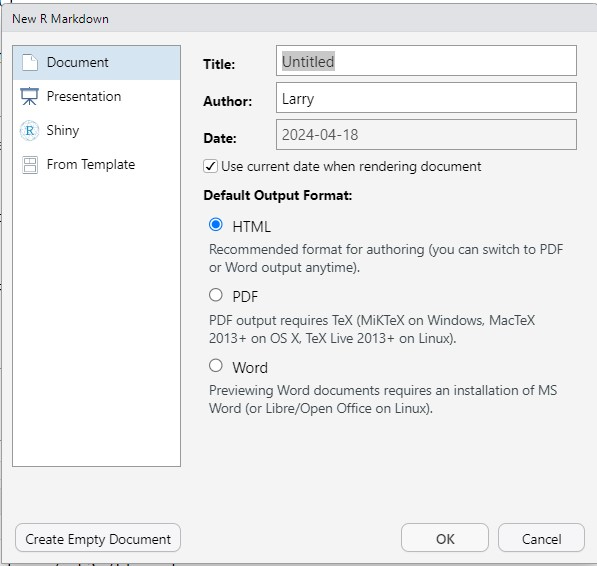
\includegraphics[width=0.6\linewidth,height=0.6\textheight]{../Document_Rmarkdown/Images/New_RMD} \end{center}

Par défaut, la page qui s'affiche est la suivante:

\begin{center}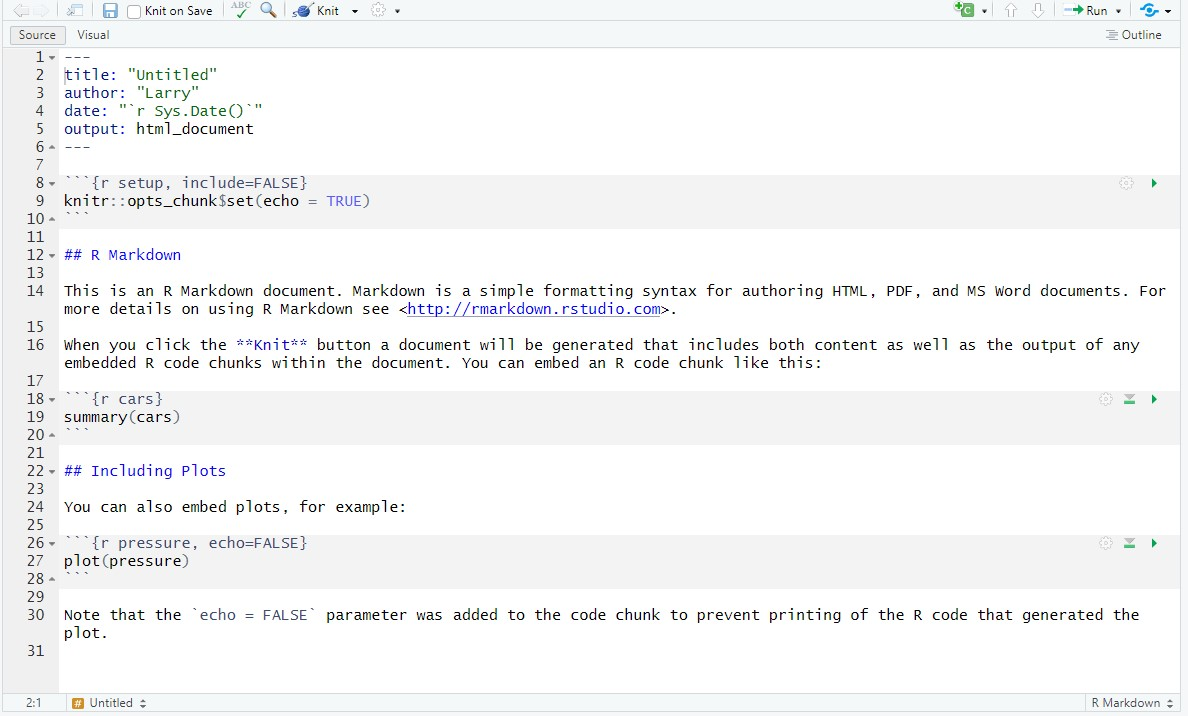
\includegraphics[width=0.6\linewidth,height=0.6\textheight]{../Document_Rmarkdown/Images/Page_defaut} \end{center}

Vous pouvez déjà y voir le titre \texttt{\#\ R\ markdown} et apercevoir
quelques chunks (pas d'inquiétude on verra ce que c'est dans la suite).

\subsubsection{En-tête YAML}\label{en-tuxeate-yaml}

L'en-tête d'un document R Markdown (parfois appelé YAML header) est
délimité par deux lignes de pointillés et contient les métadonnées du
document (titre, auteurs, options générales de mise en page\ldots). Il
contient au minimum le titre du document et le format de sortie. Il peut
être enrichi d'autres champs pour modifier certaines métadonnées (par
exemple la date) ou le style du document compilé. Voici un exemple
d'en-tête :

\begin{center}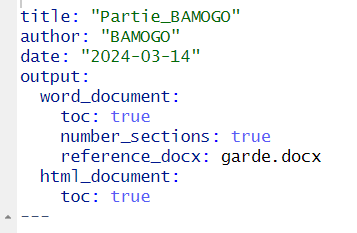
\includegraphics[width=0.5\linewidth,height=0.5\textheight]{../Document_Rmarkdown/Images/Entete} \end{center}

De nombreux champs supplémentaires peuvent être ajoutés. Par exemple,
les références bibliograhiques sont listées dans un fichier séparé et
c'est R Markdown lui-même qui se charge de la mettre en forme et de la
lier à des références dans le texte.

\subsubsection{Table des matières}\label{table-des-matiuxe8res}

Pour inclure une table des matières dans un document R Markdown généré
avec RStudio, vous pouvez utiliser l'option \texttt{toc} dans les
métadonnées YAML. Voici comment vous pouvez le faire L'option
\texttt{toc:\ true} dans le bloc YAML indique à R Markdown de générer
une table des matières ou passer menu \texttt{Edit} ensuite
\texttt{Output\ Options} et activer la partie
\texttt{table\ of\ contents}.

\begin{center}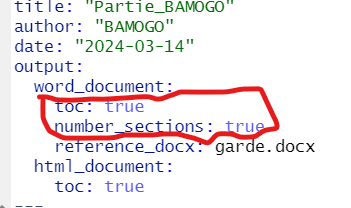
\includegraphics[width=0.5\linewidth,height=0.5\textheight]{../Document_Rmarkdown/Images/toc} \end{center}

Les titres de section sont précédés par un numéro \texttt{\#}, ce qui
indique à Markdown qu'il s'agit d'un titre de section. Markdown
convertira automatiquement ces titres en liens de la table des matières.
Chaque titre de section est également associé à un identifiant unique
(par exemple, \texttt{\#} première-section). Ces identifiants sont
utilisés dans les liens de la table des matières pour pointer vers
chaque section. Pour facilite la tache RStudio propose néanmoins une
petite interface graphique permettant de changer ces options plus
facilement. Pour cela, cliquez sur l'icône en forme d'engrenage à droite
du bouton \texttt{Knit} et choisissez \texttt{Output\ Options}.

\begin{center}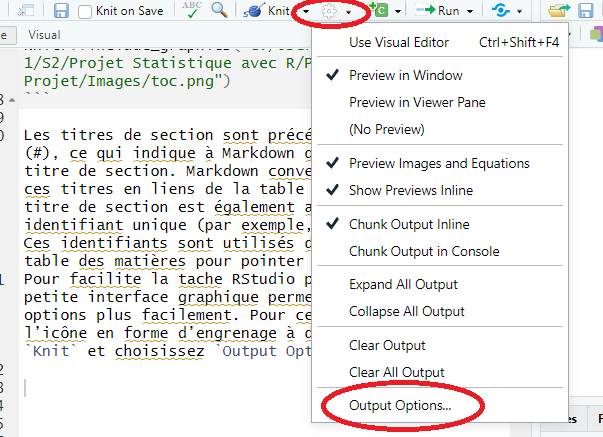
\includegraphics[width=0.5\linewidth,height=0.5\textheight]{../Document_Rmarkdown/Images/Output_option} \end{center}

\subsubsection{Les styles et thèmes}\label{les-styles-et-thuxe8mes}

Il est possible avec Rmarkdown d'importer un document word et import les
styles qui y sont et appliquer a notre document de sortir. Pour le
faire, il faut faire appel à l'option des métadonnées
\texttt{reference\_docx}. Cet option prend comme valeur le chemin de
notre fichier en question. Voici un exemple:

\begin{center}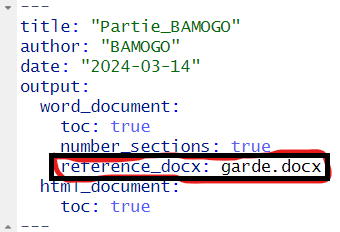
\includegraphics[width=0.5\linewidth,height=0.5\textheight]{../Document_Rmarkdown/Images/Style} \end{center}

\subsubsection{L'option params}\label{loption-params}

L'option \texttt{params} dans l'en-tête d'un chunk R Markdown est
utilisée pour spécifier des paramètres externes que vous souhaitez
passer au chunk lors de son exécution. Ces paramètres peuvent être
définis à l'extérieur du document R Markdown et injectés dans le
document au moment de son exécution. Pour illustrer son importance nous
pouvons utiliser l'exemple d'une base contemant des informations des
individus. Ces individus sont dans divers secteurs activités tel que le
commerce, l'agriculture, l'elevage, l'artisanat, etc. Nous pouvons
utiliser l'option parms au niveau de l'en-tete pour générer un rapport
pour chaque secteur d'activités. Il n'y pas de limite concernant le
nombre de paramètres à insérer.

\begin{center}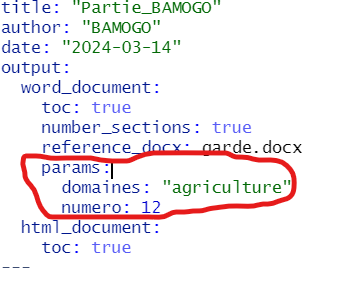
\includegraphics[width=0.5\linewidth,height=0.5\textheight]{../Document_Rmarkdown/Images/Params} \end{center}

\textbf{Application}

\begin{itemize}
\tightlist
\item
  \textbf{Préambule :}
\end{itemize}

Comme application, nous avons écrit un code R markdown qui fait
l'équivalent du publipostage sous Word.

À partir de l'echantillon ci-dessous :

\begin{center}
\includegraphics[width=1\linewidth,height=1\textheight]{../Document_Rmarkdown/Images/Echantillon_publipostage} \end{center}

Nous voulons remplacer automatiquement \textbf{Étudiant},
\textbf{Diplôme}, \textbf{Date de Graduation} et \textbf{Université} par
leurs valeurs correspondantes.

\begin{itemize}
\tightlist
\item
  \textbf{Processus et codes :}
\end{itemize}

À la base, nous avons un document nommé \textbf{\texttt{templedi}} comme
échantillon.

\begin{center}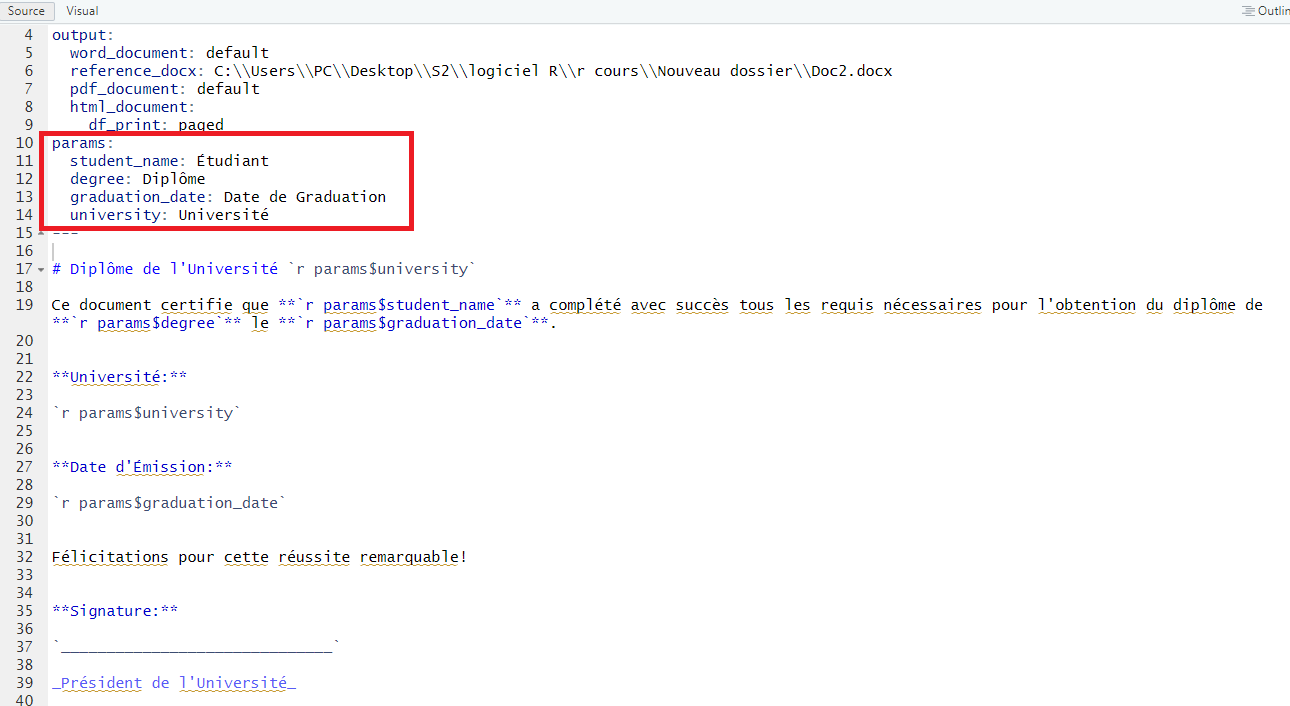
\includegraphics[width=1\linewidth,height=1\textheight]{../Document_Rmarkdown/Images/templedi} \end{center}

Dans ce document R Markdown, nous avons les paramètres
\texttt{student\_name},\texttt{degree},\texttt{graduation\_date} et
\texttt{university} qui sont insérés dans l'option
\textbf{\texttt{param}}. Ce sont eux qui à chaque fois qu'ils sont
modifiés dans l'entête YAML permettent de changer automatiquement le
document.

Pour créer des documents automatiquement, nous avons écrit un script R
qui permet de générer automatiquement les documents à l'aide de la
commande \texttt{rmarkdown::render()}; le script en question est le
suivant :

\begin{center}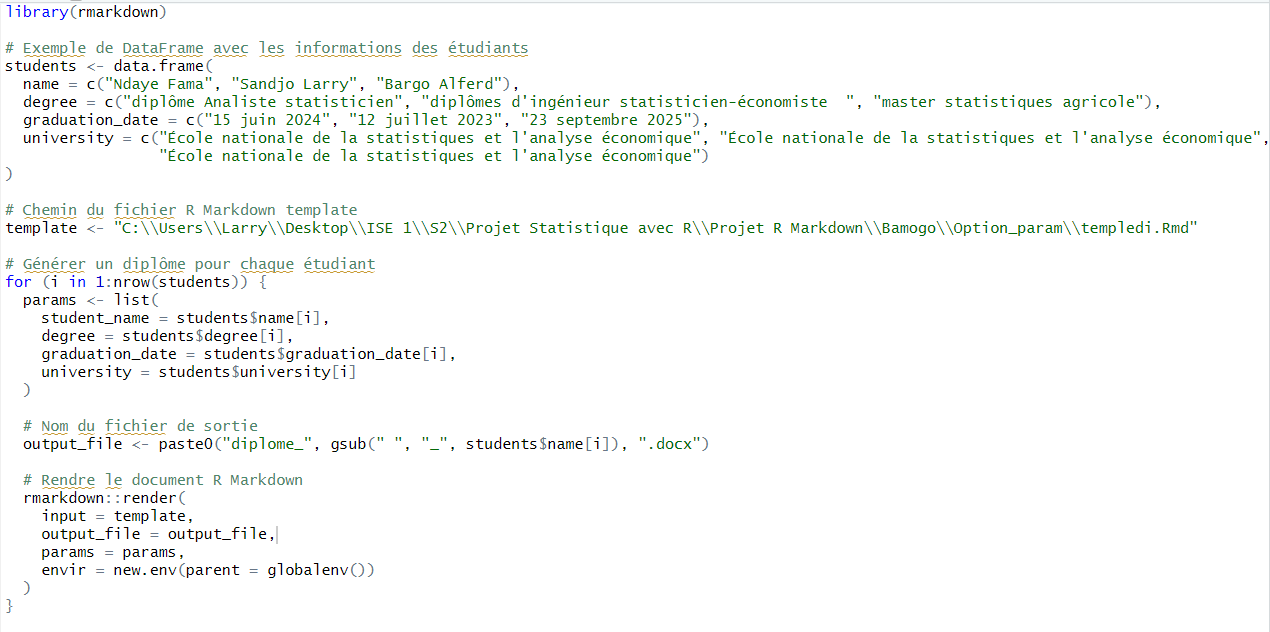
\includegraphics[width=1\linewidth,height=1\textheight]{../Document_Rmarkdown/Images/essai} \end{center}

Comme vous le constatez la variable \textbf{\texttt{student}} contient
les informations à entrer dans la partie de l'options \texttt{param}. La
boucle \texttt{for} juste en bas permet de compiler chaque document pour
les différentes informations.

\begin{itemize}
\tightlist
\item
  \textbf{Sorties :}
\end{itemize}

Après execution du script, on a les différentes sorties suivantes :

\begin{center}
\includegraphics[width=1\linewidth,height=1\textheight]{../Document_Rmarkdown/Images/Sortie_param1} \end{center}

\begin{center}
\includegraphics[width=1\linewidth,height=1\textheight]{../Document_Rmarkdown/Images/Sortie_param2} \end{center}

\begin{center}
\includegraphics[width=1\linewidth,height=1\textheight]{../Document_Rmarkdown/Images/Sortie_param3} \end{center}

On constate alors que les différentes informations apparaissent chacunes
sur son document spécifique.

\textbf{NB :} Rassurez-vous que votre script R et votre document R
markdown utilisé comme template soient dans le \textbf{même dossier}.

\subsubsection{Chunks de code}\label{chunks-de-code}

En plus du texte libre au format Markdown, un document R Markdown
contient, comme son nom l'indique, du code R. Celui-ci est inclus dans
des blocs (chunks) délimités par la syntaxe suivante :

\begin{center}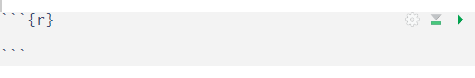
\includegraphics[width=1\linewidth,height=1\textheight]{../Document_Rmarkdown/Images/Chunk} \end{center}

Comme cette suite de caractères n'est pas très simple à saisir, vous
pouvez utiliser le menu \texttt{Insert} de RStudio et choisir le type de
chunks que vous voulez

\begin{center}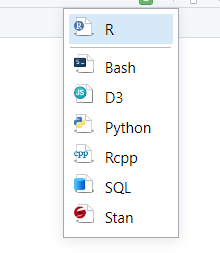
\includegraphics[width=0.3\linewidth,height=0.3\textheight]{../Document_Rmarkdown/Images/Type_chunk} \end{center}

Ou utiliser le raccourci clavier \textbf{\texttt{Ctrl+Alt+i}}. Quand
votre curseur se trouve dans un bloc, vous pouvez saisir le code R que
vous souhaitez, l'exécuter, utiliser l'autocomplétion, exactement comme
si vous vous trouviez dans un script R. Vous pouvez également exécuter
l'ensemble du code contenu dans un bloc à l'aide du raccourci clavier
\texttt{Ctrl+Maj+Entrée}. Le corps d'un document R Markdown comprend
deux types de blocs, qu'on peut alterner librement, les chunks ont deux
carcateristiques importants à savoir: + Ces chunks peuvent être nommés
(il est même recommandé de le faire) ; + Des options peuvent être
spécifiées. Ces options (détaillées plus bas) permettent par exemple de
ne pas faire figurer l'output du code dans le document final ou
inversement de ne montrer que l'output du code et non le code l'ayant
généré.

Quelques options des chunks Les options de chunk peuvent être
personnalisées avec les options \texttt{knitr}, des arguments définis
dans les \{\} de l'en-tête d'un chunk. Ci-dessus, nous utilisons cinq
arguments les plus utilisés :

\begin{center}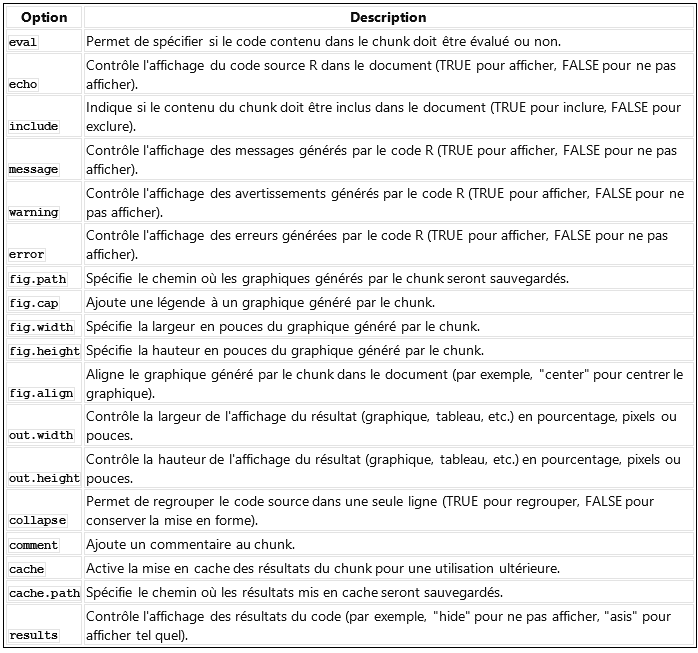
\includegraphics[width=1\linewidth,height=1\textheight]{../Document_Rmarkdown/Images/Options_chunk} \end{center}

Consultez le Guide de référence de R Markdown pour une liste complète
des options de chunk knitr. Il est possible aussi de définir des options
globales qui s'appliquent à chaque chunk de votre fichier, appelez
knitr::opts\_chunks et dans un chunk de code. Knitr traitera chaque
option que vous transmettez à \texttt{knitr::opts\_chunkset} comme un
défaut global pouvant être écrasé dans les en-têtes de chunk
individuels.

\newpage

\section{Personnalisation d'un document R
markdown}\label{personnalisation-dun-document-r-markdown}

\subsection{Les notes de bas de page}\label{les-notes-de-bas-de-page}

Markdown nous permet d'éditer des notes de bas de page. Il suffit
ajoutez tout simplement dans votre texte un numéro d'annotation, et
reprenez ce numéro en bas de votre page dans une note de bas de page.
Markdown créera alors automatiquement une ligne. L'insertion de notes de
bas de page numérotées s'effectue à l'aide de crochets \texttt{({[}{]})}
contenant un accent circonflèxe et une référence qui peut être soit un
nombre, soit un texte (mais sans espace ou autre caractère blanc).

\textbf{Application}

Le numéro de la note de bas de page est un lien qui renvoie vers la
note\footnote{\emph{L'interet de la note de bas de page}}. Une flèche de
retour est proposée pour ramener au texte lorsque le document créé est
un document html\footnote{\emph{Si le document est html}}.

\subsection{Ajout de bibliographie}\label{ajout-de-bibliographie}

Pour insérer une bibliographie dans un document R Markdown, on peut
utiliser des fichiers de style CSL (Citation Style Language) et des
logiciels comme Zotero ou Mendeley pour gérer vos références
bibliographiques. Voici une méthode générale pour le faire :

Utilisez un logiciel de gestion de références bibliographiques tel que
Zotero, Mendeley ou EndNote pour collecter et organiser vos références.
Assurez-vous d'exporter votre bibliographie dans un format compatible
CSL, tel que BibTeX (.bib) ou CSL JSON (.json).

Téléchargez un fichier de style CSL correspondant à vos besoins. CSL est
un langage de style de citation qui contrôle le format de citation et de
bibliographie dans les documents. Vous pouvez trouver des styles CSL sur
le site officiel de CSL \url{https://citationstyles.org/}.

Configurer votre document R Markdown : Dans votre document R Markdown,
vous pouvez spécifier le style de citation et la bibliographie à
utiliser dans le YAML en-tête. Assurez-vous que le chemin vers votre
fichier de bibliographie (biblio.bib) et votre fichier de style CSL
(style.csl).

Configurer votre document R Markdown : Dans votre document R Markdown,
vous pouvez spécifier le style de citation et la bibliographie à
utiliser dans le YAML en-tête. Assurez-vous que le chemin vers votre
fichier de bibliographie (biblio.bib) et votre fichier de style CSL
(style.csl).

\subsection{Insertion de tableau}\label{insertion-de-tableau}

Pour insérer des tableaux basiques dans un document RMarkdown, on peut
utiliser la syntaxe Markdown pour créer des tableaux simples.

La syntaxe Markdown permet de créer un tableau en utilisant des barres
verticales \texttt{\textbar{}} pour séparer les colonnes et des tirets -
pour séparer les lignes.

Pour personnaliser votre tableau en ajoutant des éléments Markdown
supplémentaires, utilisez deux points : dans les barres verticales pour
aligner le texte dans les colonnes. Par exemple :---: pour centrer, :---
pour aligner à gauche, ---: pour aligner à droite.

Après avoir tricoté le document RMarkdown, le tableau sera formaté
correctement dans la sortie finale, que ce soit dans un fichier PDF,
HTML ou autre, en fonction du format que vous avez choisi pour votre
document. Pour des fonctionnalités plus avancées ou de tableaux plus
complexes, on pourra également utiliser des packages R spécifiques,
comme kable() de knitr, pour créer et personnaliser des tableaux à
partir de données R.

\textbf{Application}

Par exemple, lorsqu'on entre le code ci-dessous,

\begin{center}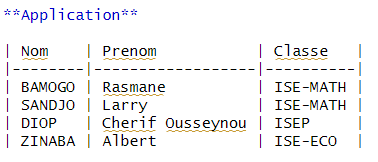
\includegraphics[width=0.7\linewidth,height=0.7\textheight]{../Document_Rmarkdown/Images/code_tableau} \end{center}

On obtient la sortie suivante.

\begin{longtable}[]{@{}lll@{}}
\toprule\noalign{}
Nom & Prenom & Classe \\
\midrule\noalign{}
\endhead
\bottomrule\noalign{}
\endlastfoot
BAMOGO & Rasmane & ISE-MATH \\
SANDJO & Larry & ISE-MATH \\
DIOP & Cherif Ousseynou & ISEP \\
ZINABA & Albert & ISE-ECO \\
\end{longtable}

Il est aussi possible de faire des tableaux à l'aide des codes R à
partir des chunks. Les fonctions telles que \texttt{kable()} de la
librarie \texttt{knitr} et \texttt{tbl\_summary()} de \texttt{gtsummary}
sont vivement conseillées.

\subsection{Insertion de lien}\label{insertion-de-lien}

R markdown permet de créer des liens qui facilite la navigation vers le
web ,local ou même dans notre document.

\begin{itemize}
\tightlist
\item
  \textbf{Insersion du lien web :}
\end{itemize}

La syntaxes est la suivante entre crochet le titre du lien suivis d'une
parenthèse contenant le lien web.

\textbf{Exemple :}

Le code suivant :

\begin{center}
\includegraphics[width=0.7\linewidth,height=0.7\textheight]{../Document_Rmarkdown/Images/Lien_Zotero} \end{center}

Permet d'avoir le lien suivant : \href{https://www.zotero.org/}{Lien
vers zoreto}

\begin{itemize}
\tightlist
\item
  \textbf{Lien vers un fichier local :}
\end{itemize}

La syntaxe est la suivante; entre crochet le titre du lien suivis d'une
parenthèse contenant le chemin d'accès au document

\textbf{Exemple :}

Voici une photo du code :

\begin{center}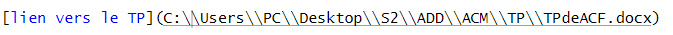
\includegraphics[width=0.7\linewidth,height=0.7\textheight]{../Document_Rmarkdown/Images/Lien_Local} \end{center}

\href{C:/Users/Larry/Desktop/ISE\%201/S2/Projet\%20Statistique\%20avec\%20R/Projet\%20R\%20Markdown/Plan_de_travail_R_Markdown\%5B1\%5D.docx}{lien
vers le TP}

\begin{itemize}
\tightlist
\item
  \textbf{Lien vers un titre du document :}
\end{itemize}

La syntaxe est la suivantel; entre crochet contenant le titre du
document suivi d'une parenthèse contenant le titre mais le titre doit
être début par un \texttt{\#}:

\begin{center}
\includegraphics[width=0.7\linewidth,height=0.7\textheight]{../Document_Rmarkdown/Images/Lien_vers_titre} \end{center}

\hyperref[ux5cux2520Insertionux5cux2520dux27unux5cux2520lienux5cux2520dansux5cux2520leux5cux2520documentux5cux2520rmarkdown]{Retour
vers l'insertion}

Dans tous les cas le titre n'est pas obligatoire mais au cas où il n'y a
pas de titre les crochets doivent être mis et laissier vide

\subsection{Insertion d'images}\label{insertion-dimages}

Pour insérer des images dans un document RMarkdown, la syntaxe suivante
:

\texttt{!{[}{]}(\%22chemin//vers\%20//votre//image.jpg)}.

Pour ce faire il faut s'assurer que le nom de l'image que vous avez mis
est le bon, par exemple ici ``imge.jpg'' dans l'exemple précedent.

Lorsque vous rendrez votre document RMarkdown, l'image sera incorporée
dans le document rendu. Assurez-vous également que vous avez les
packages nécessaires pour le rendu de votre document RMarkdown avec des
images, comme knitr et rmarkdown, installés et chargés dans votre
environnement R.\\
Pour ajouter une description de l'image, pour pouvez insérer la
description dans les crochets. Par exemple {[}``description''{]}.

\textbf{Application}

Le code R markdown suivant permet d'obtenir la sortie ci-dessous :

\begin{center}
\includegraphics[width=0.8\linewidth,height=0.8\textheight]{../Document_Rmarkdown/Images/code_image} \end{center}

\begin{figure}
\centering
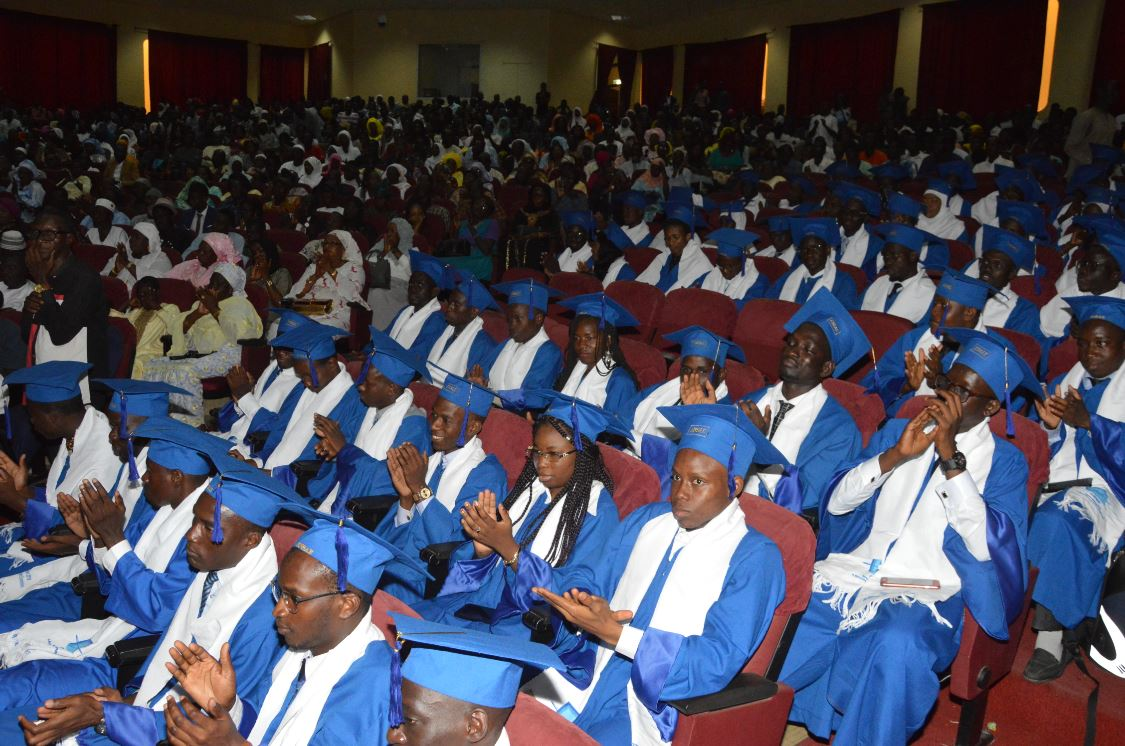
\includegraphics{ENSAE_Image.JPG}
\caption{Une sortie de promotion à l'ENSAE}
\end{figure}

Il est aussi possible d'insérer des images à partir des chunks à l'aide
de la fonction \texttt{include\_graphics()} de la librarie
\texttt{knitr}. En procédant ainsi, il est alors possible de contrôler
la largeur de l'image à l'aide de l'option de chunk \texttt{out.width}
et la longueur de par l'option \texttt{out.height}.

\newpage

\subsection{Equations mathématiques}\label{equations-mathuxe9matiques}

Pour insérer des équations mathématiques dans un document RMarkdown, on
peut utiliser la syntaxe LaTeX, qui est largement utilisée pour la mise
en forme mathématique. Quelques façons d'insérer des équations
mathématiques :

\subsubsection{Equations en ligne}\label{equations-en-ligne}

Pour inclure des équations mathématiques directement dans le texte, on
peut les entourer de symboles \$.

\textbf{Exemple :}

Lorsque l'on insère le code lateX suivant \texttt{\$f(x)\ =\ x+y\$} on
obtient la sortie suivante : \(f(x) = x+y\)

\subsubsection{Équations centrées}\label{uxe9quations-centruxe9es}

Pour afficher des équations mathématiques sur leur propre ligne, vous
pouvez les entourer de symboles \texttt{\$\$}.

\textbf{Exemple :}

Le code suivant permet d'obtenir la sortie plus bas il utilise la balise
LateX
\texttt{\textbackslash{}begin\{aligned\}...\textbackslash{}end\{aligned\}}:

\begin{verbatim}
$$\begin{aligned}
        \sum_{i=1}^{n}x_{i}&=-\dfrac{a_{n-1}}{a_{n}}\\
        \sum_{1\leq i<j\leq n}x_{i}x_{j}&=+\dfrac{a_{n-2}}{a_{n}}\\
        \sum_{1\leq i<j<k\leq n}&=-\dfrac{a_{n-3}}{a_{n}}\\
        \vdots &\\
        \sum_{1\leq i_{1}<i_{2}<\cdots <i_{P}\leq n}x_{i_{1}}x_{i_{2}}\cdots x_{i_{P}}&=(-1)^{p}\dfrac{a_{n-p}}{a_{n}}\\
        \vdots&\\
        \prod_{i=1}^{n}x_{i}&=(-1)^{n}\dfrac{a_{0}}{a_{n}}
    \end{aligned}$$
\end{verbatim}

\textbf{Sortie :}

\[\begin{aligned}
        \sum_{i=1}^{n}x_{i}&=-\dfrac{a_{n-1}}{a_{n}}\\
        \sum_{1\leq i<j\leq n}x_{i}x_{j}&=+\dfrac{a_{n-2}}{a_{n}}\\
        \sum_{1\leq i<j<k\leq n}&=-\dfrac{a_{n-3}}{a_{n}}\\
        \vdots &\\
        \sum_{1\leq i_{1}<i_{2}<\cdots <i_{P}\leq n}x_{i_{1}}x_{i_{2}}\cdots x_{i_{P}}&=(-1)^{p}\dfrac{a_{n-p}}{a_{n}}\\
        \vdots&\\
        \prod_{i=1}^{n}x_{i}&=(-1)^{n}\dfrac{a_{0}}{a_{n}}
    \end{aligned}\]

Il est aussi possible d'utiliser les codes LateX
\texttt{\textbackslash{}begin\{equation\}...\textbackslash{}end\{equation\}}

\textbf{Exemple :}

\begin{equation}
E = mc^2
\end{equation}

\subsubsection{Notation LaTeX}\label{notation-latex}

On peut egalement utiliser la notation LaTeX pour écrire des expressions
mathématiques plus complexes, telles que les fractions, les indices, les
exposants, les racines carrées, etc.

\textbf{Exemple : Une division euclidienne}

Avec le code lateX suivant on obtient une la division euclidienne plus
bas.

\begin{center}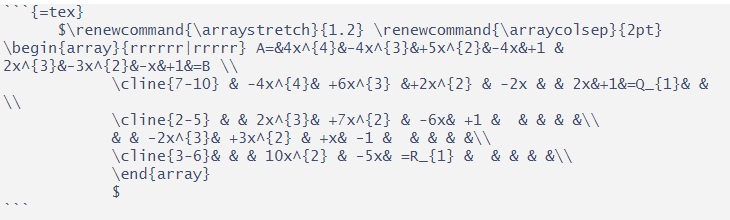
\includegraphics[width=0.8\linewidth,height=0.8\textheight]{../Document_Rmarkdown/Images/division_euclidienne} \end{center}

      $\renewcommand{\arraystretch}{1.2} \renewcommand{\arraycolsep}{2pt} \begin{array}{rrrrrr|rrrrr} A=&4x^{4}&-4x^{3}&+5x^{2}&-4x&+1 & 2x^{3}&-3x^{2}&-x&+1&=B \\  
            \cline{7-10} & -4x^{4}& +6x^{3} &+2x^{2} & -2x & & 2x&+1&=Q_{1}& & \\ 
            \cline{2-5} & & 2x^{3}& +7x^{2} & -6x& +1 &  & & & &\\
            & & -2x^{3}& +3x^{2} & +x& -1 &  & & & &\\
            \cline{3-6}& & & 10x^{2} & -5x& =R_{1} &  & & & &\\
            \end{array}
            $ 

\subsection{Packages et extensions}\label{packages-et-extensions}

La création d'un modèle (ou Template) dans RMarkdown vous permet de
définir une structure de document prédéfinie avec des paramètres par
défaut, des styles personnalisés, des en-têtes, des pieds de page, etc.
Voici comment créer un modèle RMarkdown :

\subsubsection{Création du modèle}\label{cruxe9ation-du-moduxe8le}

\begin{enumerate}
\def\labelenumi{\arabic{enumi}.}
\item
  Commencez par créer un nouveau document RMarkdown dans RStudio.
\item
  Personnalisez ce document selon vos besoins : définissez les en-têtes,
  les pieds de page, les styles CSS, les balises LaTeX personnalisées,
  etc.
\item
  Enregistrez ce document dans un répertoire spécifique que vous pouvez
  facilement retrouver.
\end{enumerate}

\textbf{Exemple d'une sortie d'un modèle :}

\begin{center}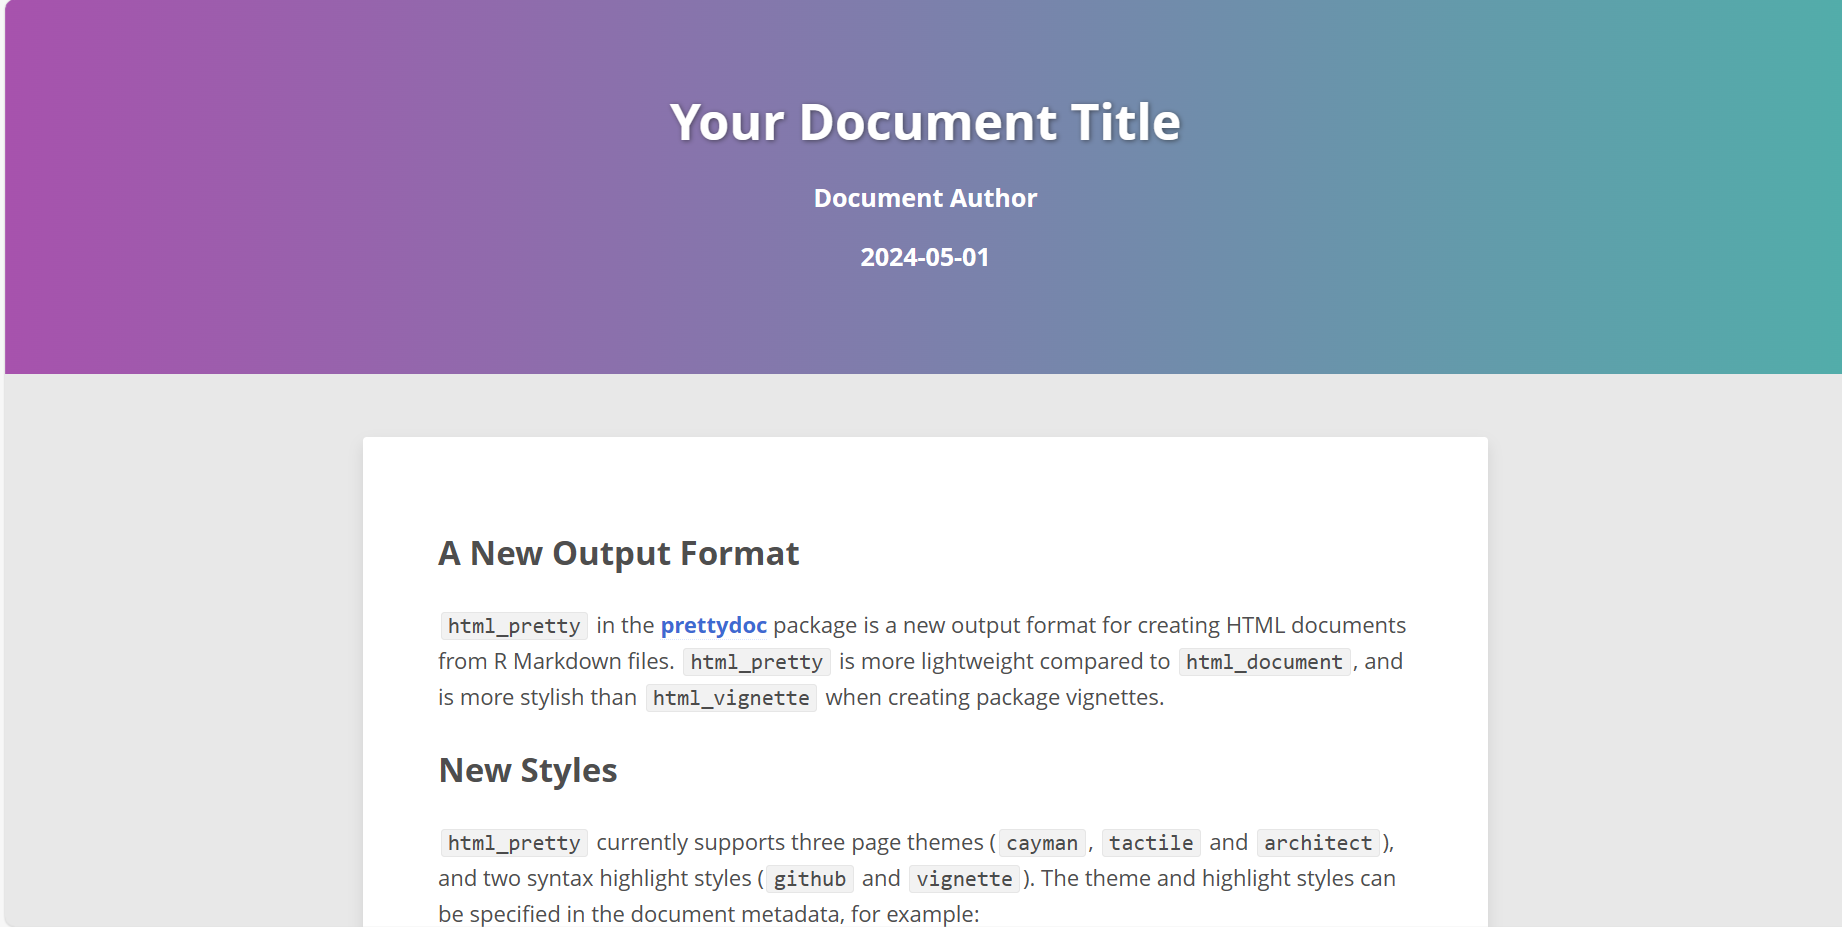
\includegraphics[width=1\linewidth,height=1\textheight]{../Document_Rmarkdown/Images/Template_github} \end{center}

Ce type de modèle peut être facilement optenu sur le site :
\url{https://github.com/yixuan/prettydoc/?tab=readme-ov-file}

\subsubsection{Utilisation du modèle}\label{utilisation-du-moduxe8le}

Pour utiliser ce modèle lors de la création d'un nouveau document
RMarkdown :

\begin{enumerate}
\def\labelenumi{\arabic{enumi}.}
\item
  Ouvrez RStudio.
\item
  Sélectionnez ``File'' \textgreater{} ``New File'' \textgreater{} ``R
  Markdown\ldots{}''.
\item
  Choisissez ``From Template'' et sélectionnez le modèle que vous avez
  créé.
\end{enumerate}

\begin{center}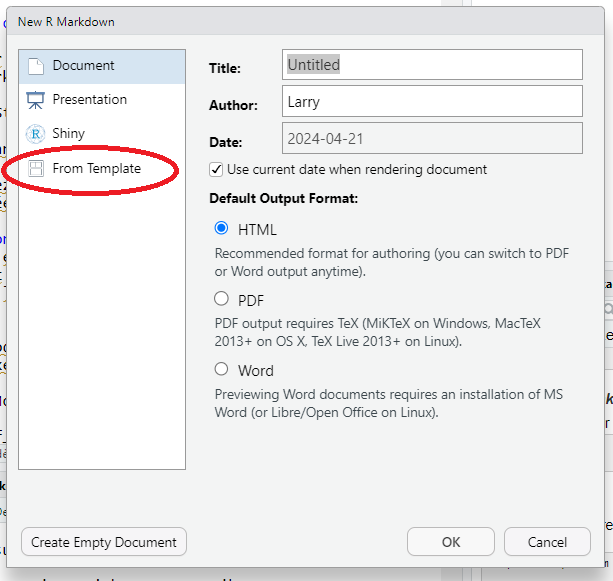
\includegraphics[width=1\linewidth,height=1\textheight]{../Document_Rmarkdown/Images/From_template} \end{center}

\subsubsection{Personnalisation
supplémentaire}\label{personnalisation-suppluxe9mentaire}

Nous pouvons également personnaliser davantage notre modèle en y
ajoutant des paramètres YAML spécifiques, tels que des options pour les
citations bibliographiques, le format de sortie, etc.

\textbf{Exemple de modèle YAML :}

Voici un exemple de YAML pour un modèle RMarkdown :

--- title: ``Mon Modèle RMarkdown''

output: pdf\_document:

toc: true

number\_sections: true

fig\_caption: true

html\_document:

toc: true

toc\_float: collapsed: false

code\_folding: hide ---

\textbf{Utilisation de données dynamiques :}

Vous pouvez également créer des modèles qui intègrent des données
dynamiques. Par exemple, vous pouvez utiliser des paramètres YAML pour
spécifier des titres ou des noms d'auteurs qui seront remplis à la
création du document.

En résumé, la création d'un modèle RMarkdown implique la
personnalisation d'un document RMarkdown selon vos besoins, puis la
sauvegarde de ce document dans un répertoire spécifique. Vous pouvez
ensuite utiliser ce modèle comme base pour créer de nouveaux documents
RMarkdown en sélectionnant ``From Template'' lors de la création d'un
nouveau document dans RStudio.

\subsection{Compléments}\label{compluxe9ments}

\subsubsection{R markdown Cheat Sheet}\label{r-markdown-cheat-sheet}

Vous pouvez avoir la liste quasi complète des balises R Markdown en
allant sur le site

\url{https://www.rstudio.com/wp-content/uploads/2015/02/rmarkdown-cheatsheet.pdf}

Il est aussi possible d'accéder aux références rapides de R markdown
proposé par la page d'aide de R. Pour cela, il suffit d'aller sur
\texttt{Help}, ensuite de cliquer sur
\texttt{Markdown\ Quick\ Reference}. La page d'aide de R s'ouvre alors
avec l'ensemble des références pour R markdown.

\begin{center}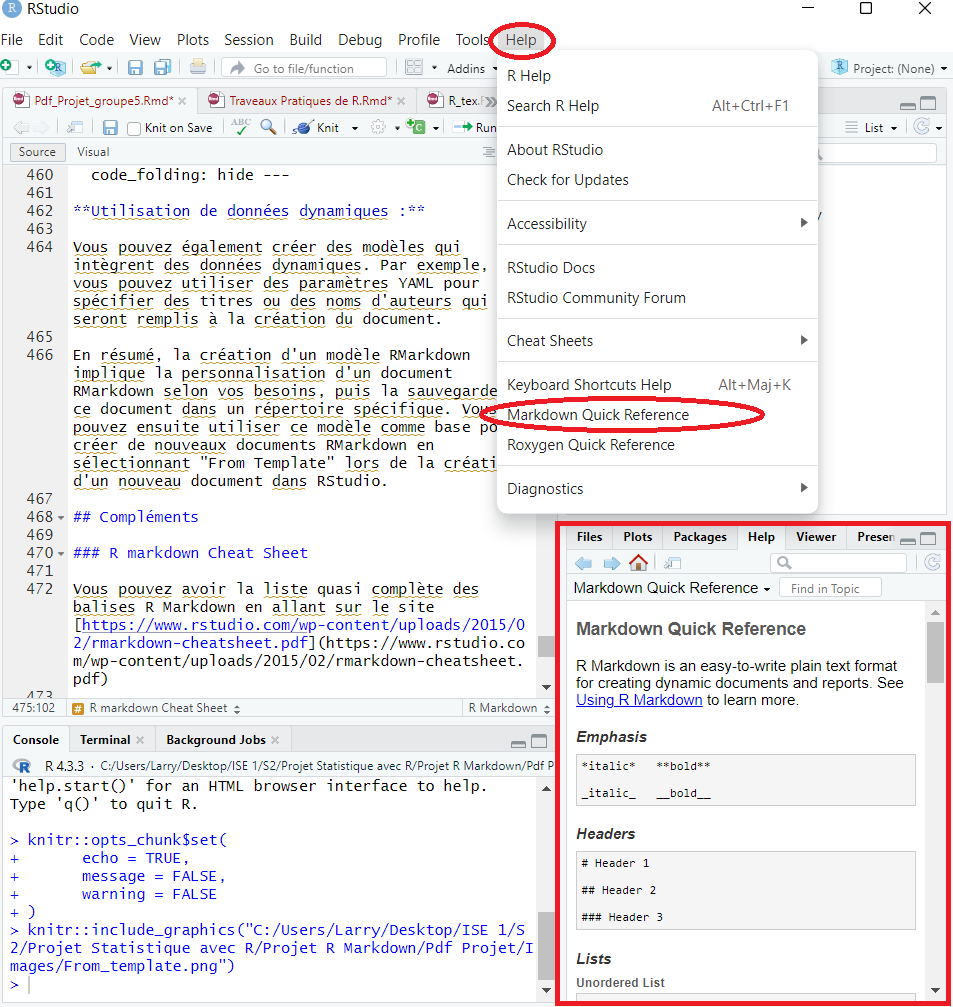
\includegraphics[width=0.7\linewidth,height=0.7\textheight]{../Document_Rmarkdown/Images/References_markdown} \end{center}

\subsubsection{Le visual de R Markdown.}\label{le-visual-de-r-markdown.}

Dans R Markdown, vous pouvez utiliser le \texttt{visual} pour effectuer
de nombreuses tâches sans avoir à retenir toutes ces balises R markdown.
Cet espace , qui ressemble beaucoup à celui de word, vous offre un
ensemble de fonctionnalités qui écrit des balises R Markdown à votre
place.

Pour Y accéder, il sufft de cliquer sur \texttt{Visual} à côté de
\texttt{source}.

\begin{center}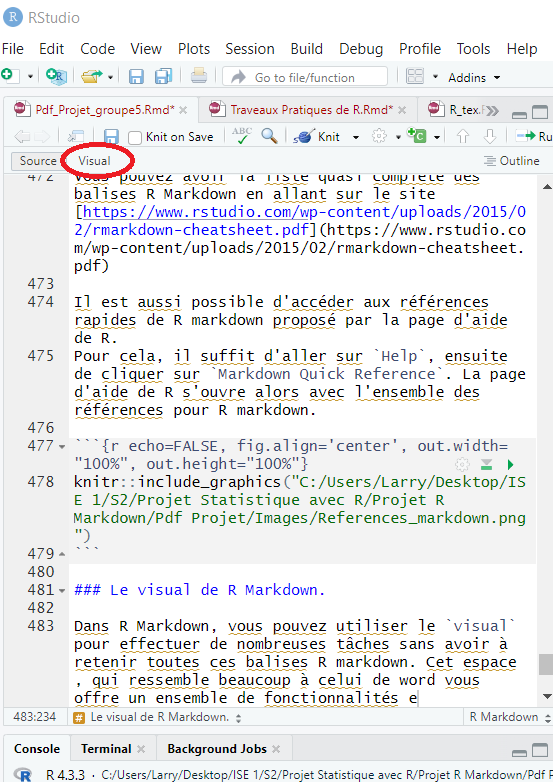
\includegraphics[width=0.6\linewidth,height=0.6\textheight]{../Document_Rmarkdown/Images/Visual} \end{center}

Vous pouvez ensuite utiliser l'ensemble des fonctionnalités telles que
mettre en gras, mettre en italique, insérer des images, des tableaux,
etc.

\begin{center}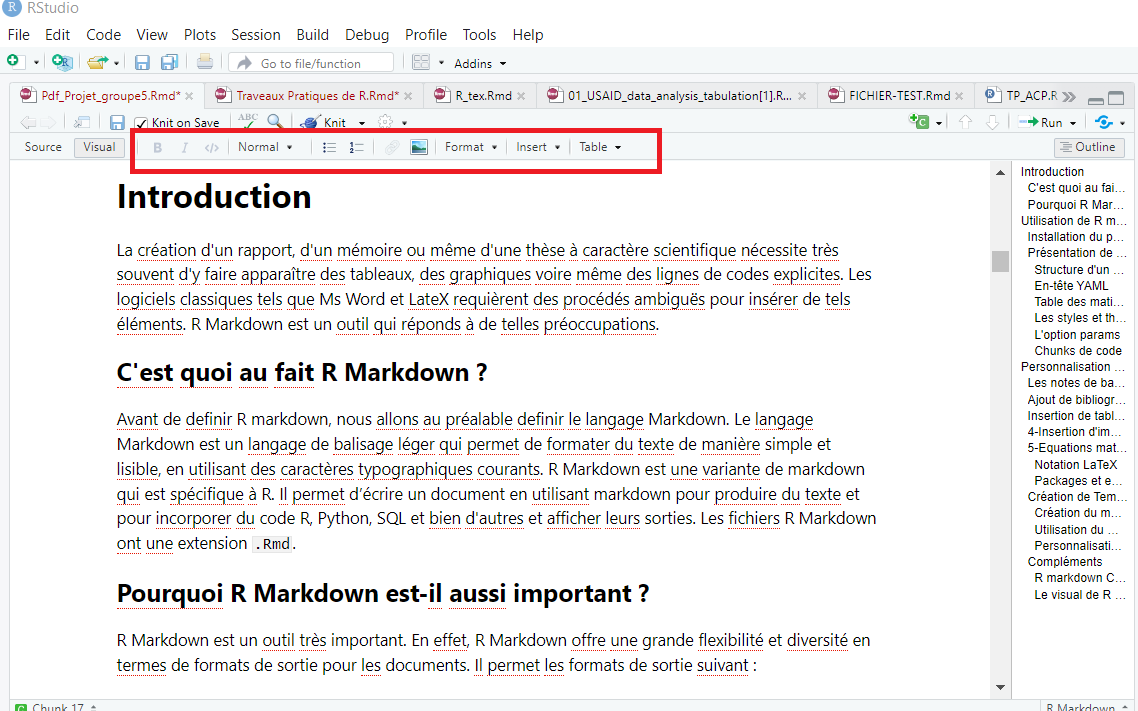
\includegraphics[width=1\linewidth,height=1\textheight]{../Document_Rmarkdown/Images/Le_Visual} \end{center}

\subsubsection{Rapport rapide à partir d'un script
R}\label{rapport-rapide-uxe0-partir-dun-script-r}

Si vos analyses sont présentes dans un script R et que ce script
contient tout le nécessaire pour la réalisation de votre analyse
(i.e.~chargement des données et des packages requis), vous pouvez très
facilement réaliser un rapport rapide au format HTML, Word ou PDF,
contenant à la fois votre code et les sorties associées.

Il suffit de cliquer sur l'icône compile report dans le quadrant
supérieur gauche.

\begin{center}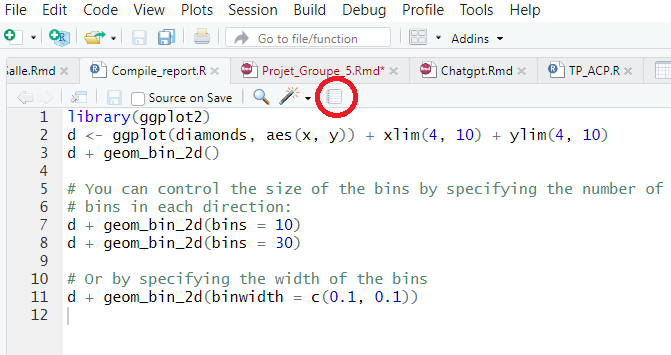
\includegraphics[width=1\linewidth,height=1\textheight]{../Document_Rmarkdown/Images/Compile_report} \end{center}

Une autre façon de faire cela est d'utiliser la commande
\texttt{rmarkdown::render("nom\_script.R")}

\newpage

\section{Formats de sortie avec R
Markdown}\label{formats-de-sortie-avec-r-markdown}

\subsection{Creation beamer}\label{creation-beamer}

Une fois que le logiciel ouvert, vous pouvez suivre les étapes suivantes
pour créer le beamer :

\begin{Shaded}
\begin{Highlighting}[]
\NormalTok{past }\OtherTok{\textless{}{-}}\NormalTok{ here}\SpecialCharTok{::}\FunctionTok{here}\NormalTok{()}
\NormalTok{image\_1 }\OtherTok{\textless{}{-}} \FunctionTok{paste0}\NormalTok{(past,}\StringTok{"/image\_1.png"}\NormalTok{)}
\NormalTok{image\_2 }\OtherTok{\textless{}{-}} \FunctionTok{paste0}\NormalTok{(past,}\StringTok{"/image\_2.png"}\NormalTok{)}
\NormalTok{image\_3 }\OtherTok{\textless{}{-}} \FunctionTok{paste0}\NormalTok{(past,}\StringTok{"/image\_3.png"}\NormalTok{)}
\end{Highlighting}
\end{Shaded}

\subsubsection{Etapes 1 :}\label{etapes-1}

\begin{figure}
\centering
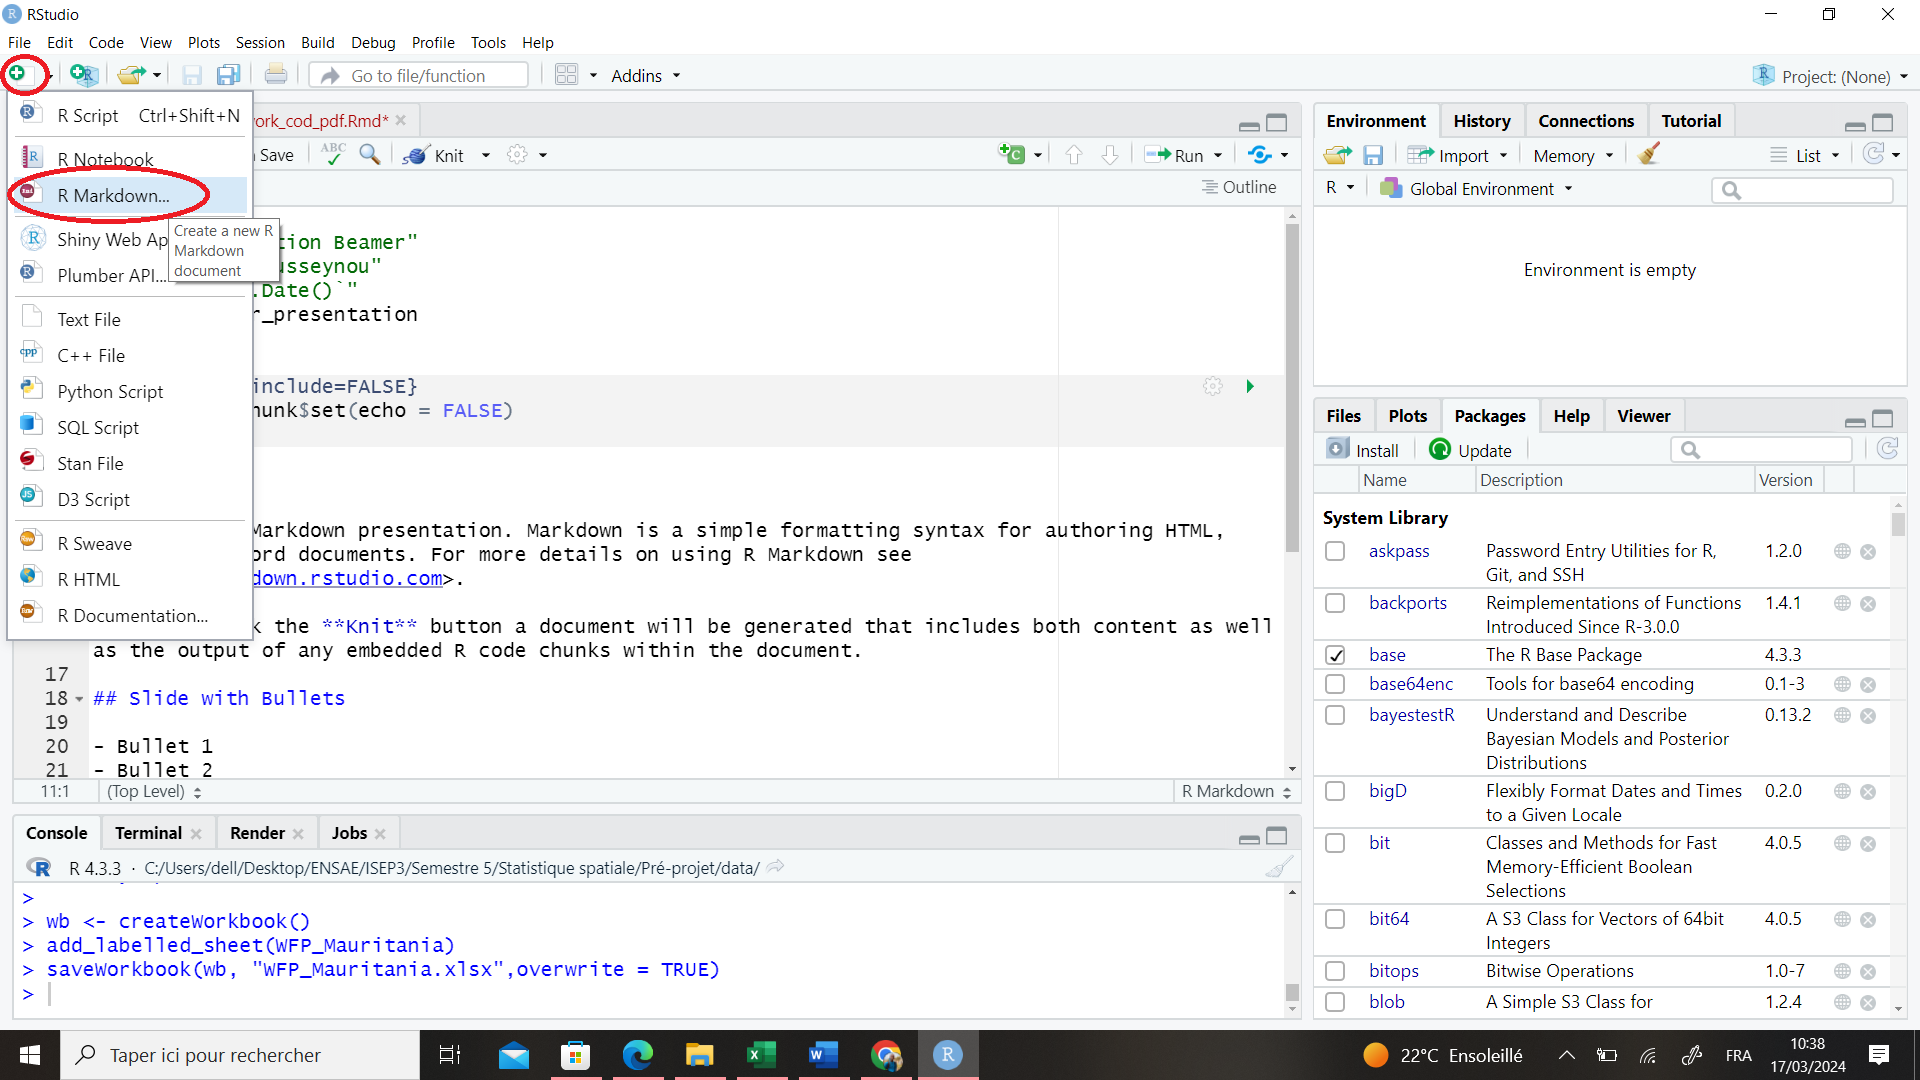
\includegraphics[width=3.64583in,height=\textheight]{image_1}
\caption{première étape création beamer}
\end{figure}

\subsubsection{Etapes 2 :}\label{etapes-2}

\begin{figure}
\centering
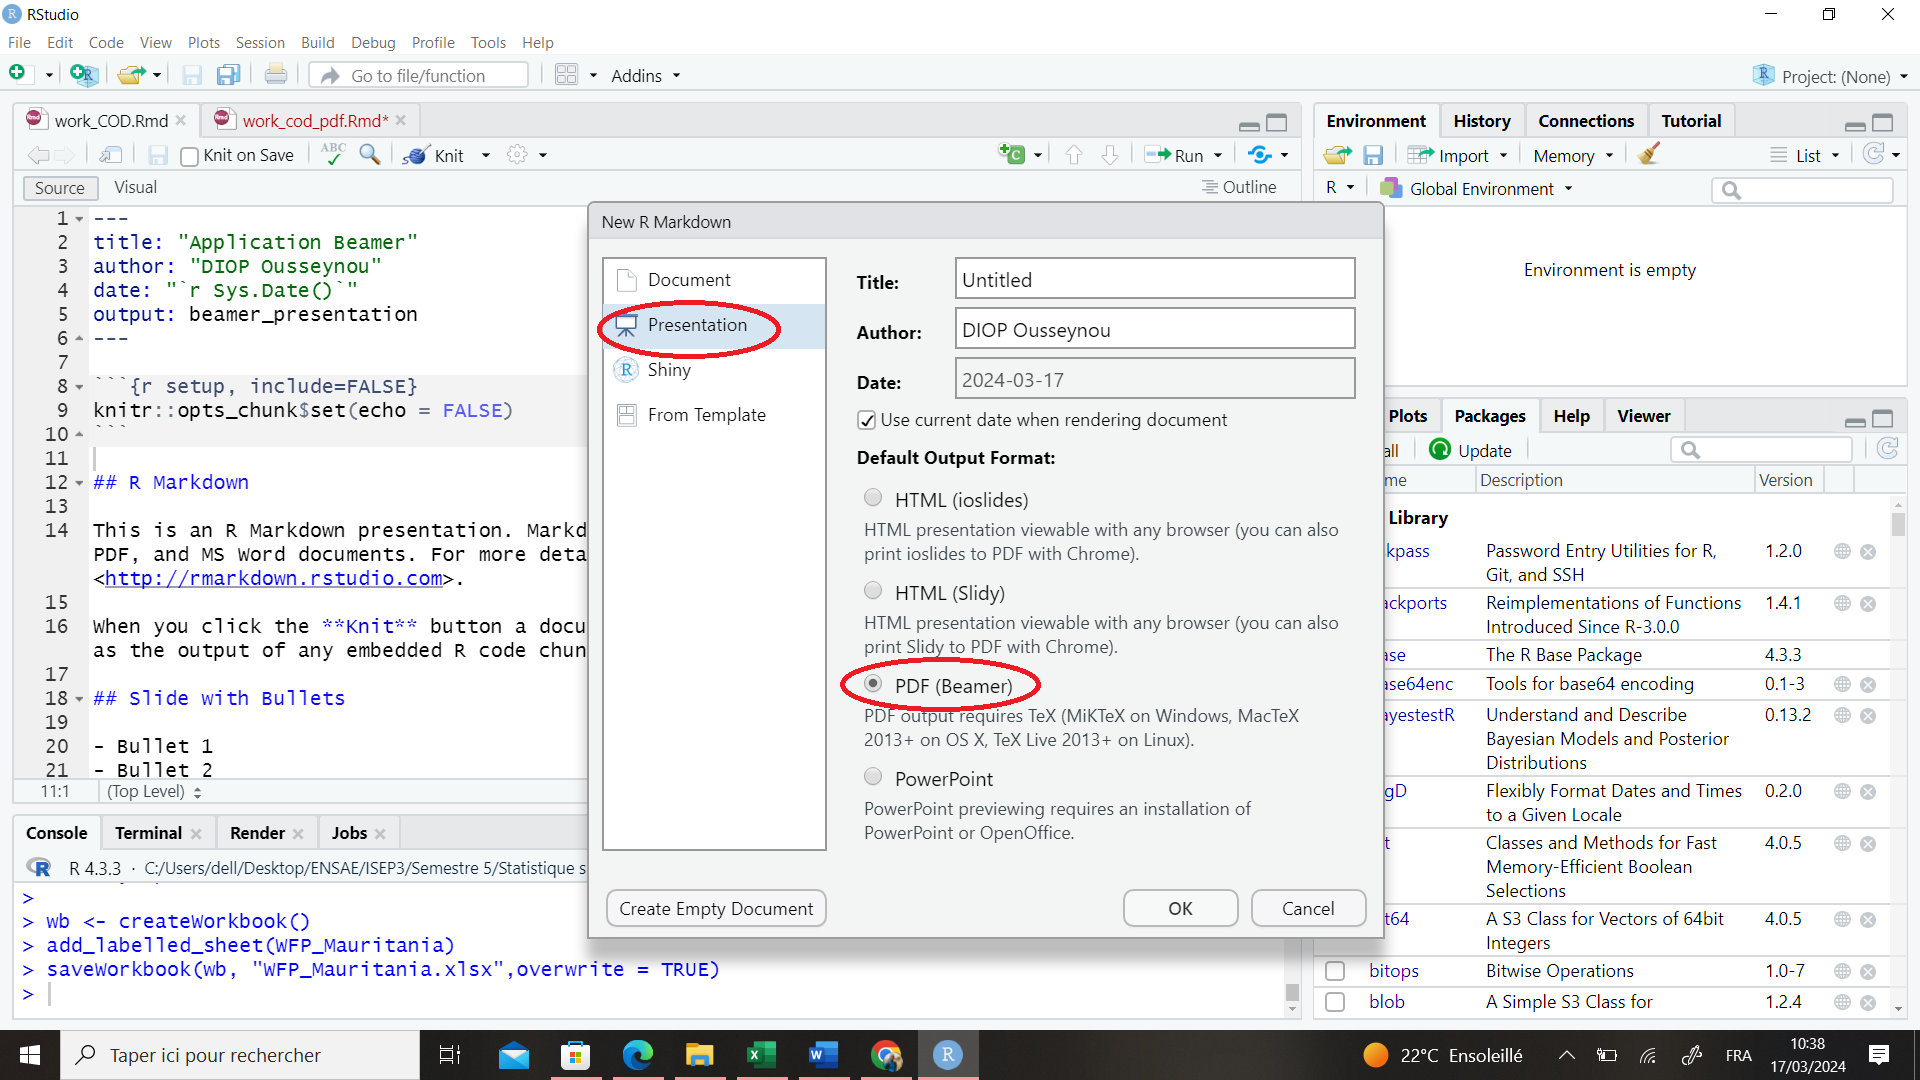
\includegraphics[width=4.16667in,height=\textheight]{image_2}
\caption{deuxieme étape création beamer}
\end{figure}

\newpage

\subsubsection{Etapes 3 :}\label{etapes-3}

\begin{figure}
\centering
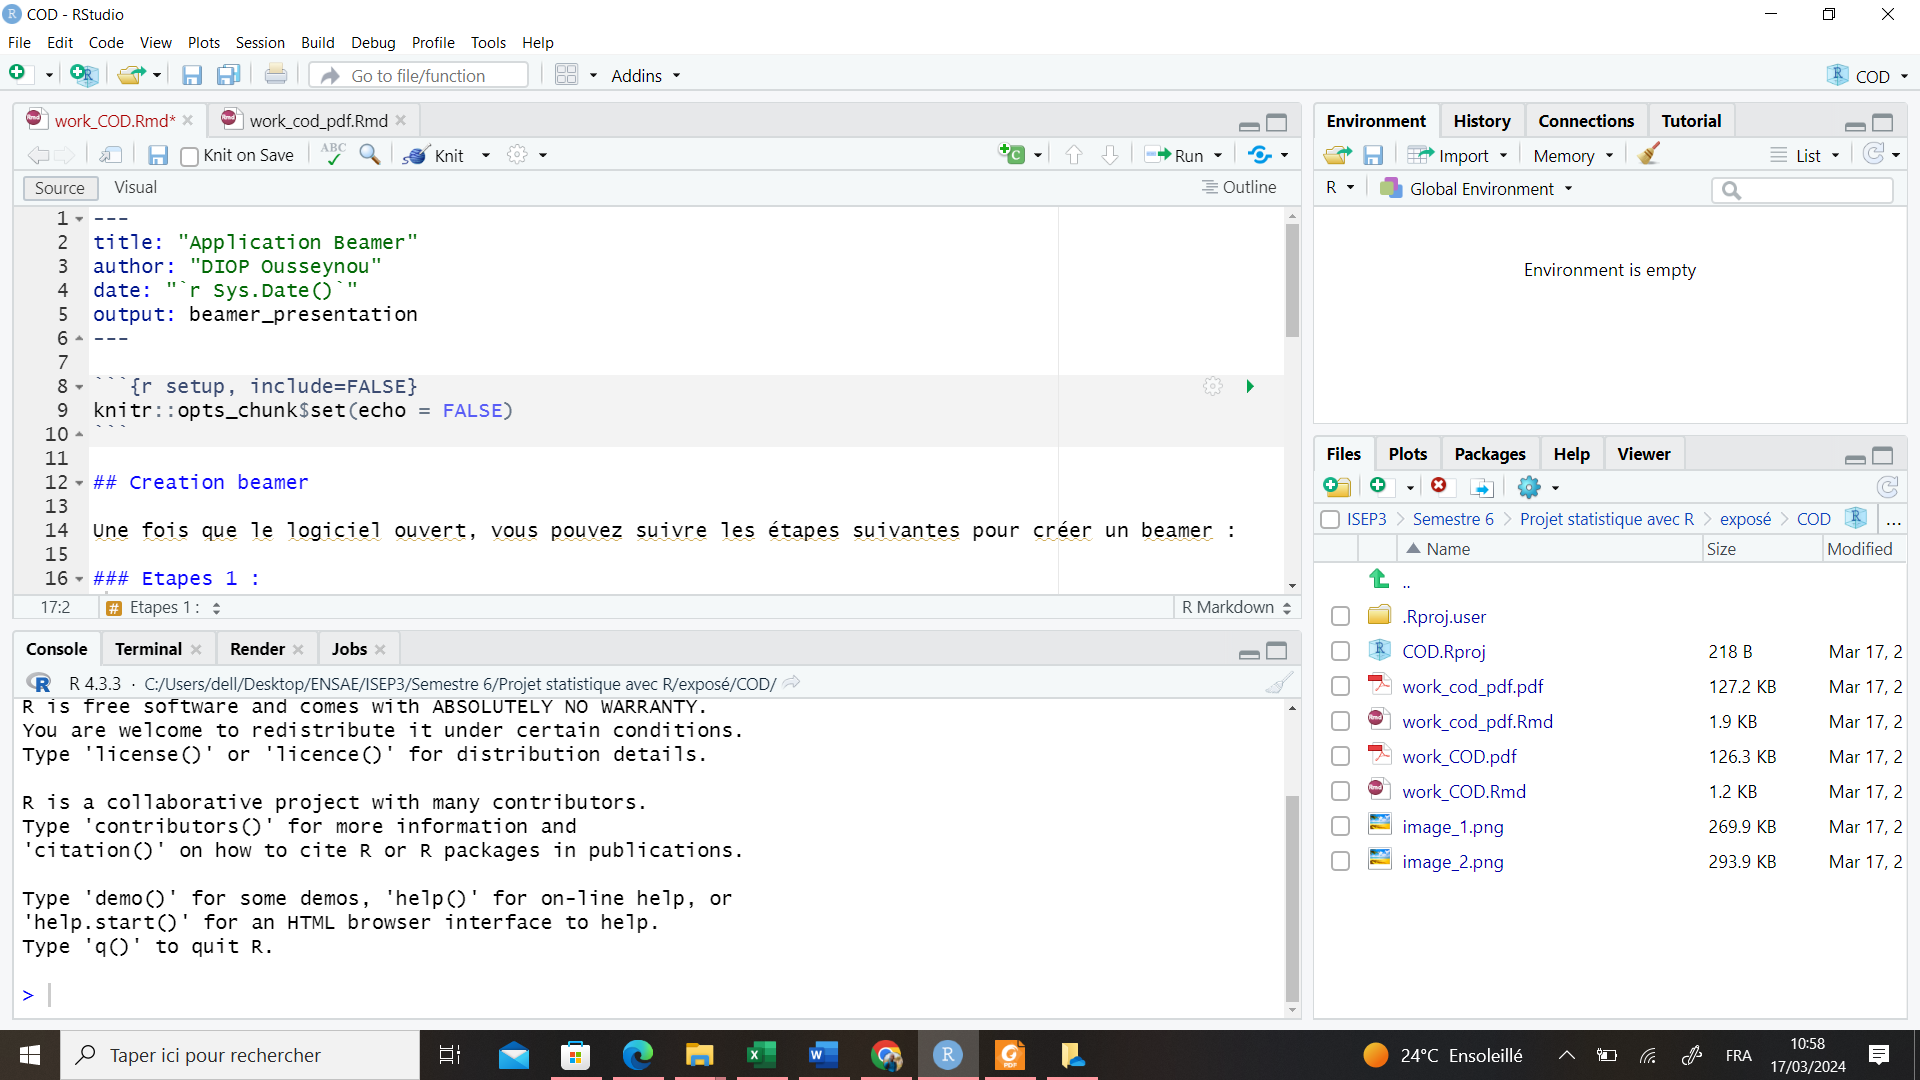
\includegraphics[width=4.16667in,height=\textheight]{image_3}
\caption{troisième étape création beamer}
\end{figure}

\subsection{Personnaliser le beamer}\label{personnaliser-le-beamer}

Aprés la création du beamer, le fichier a un format simple. Il est
possible de personnaliser la sortie.

\subsubsection{Thèmes :}\label{thuxe8mes}

Le Beamer offre une gamme de thèmes préconfigurés pour personnaliser la
présentation, parmi lesquels on retrouve : AnnArbor, Antibes, Bergen,
Berkeley, Berlin, CambridgeUS, Frankfurt, etc.

De plus, il propose également une palette de couleurs prédéfinies telles
que : bleu, vert, cyan, magenta, jaune, noir, blanc, etc.

La matrice des thèmes et des couleurs est définie sur le site :
\href{https://bookdown.org/yihui/rmarkdown/beamer-presentation.html}{\emph{Thèmes
\& couleurs beamer}}.

\begin{center}\rule{0.5\linewidth}{0.5pt}\end{center}

\subsubsection{Thème et couleur:}\label{thuxe8me-et-couleur}

Pour ajouter un thème et une couleur, il suffit d'ajouter le syntaxe au
niveau de l'output (YAML) :

\begin{itemize}
\item
  theme : ``\emph{nom\_theme}''
\item
  colortheme : ``\emph{nom\_couleur}''
\end{itemize}

\subsubsection{Exemple :}\label{exemple}

title: ``Application Beamer''

author: ``DIOP Ousseynou''

date: ``2024-05-23''

output: ''

beamer\_presentation:''

\begin{verbatim}
theme: "Madrid"" 

colortheme: "dolphin"
\end{verbatim}

\subsection{Niveau coulissant :}\label{niveau-coulissant}

Le niveau de coulissant correspond à la hiérarchie des titres dans une
présentation Beamer. Dans RMarkdown, le paramètre \emph{slide\_level}
contrôle cette structuration en spécifiant le niveau de titre qui doit
générer une nouvelle diapositive dans la sortie Beamer.

\subsubsection{Remarque}\label{remarque}

Par défaut, \emph{slide\_level} est fixé à 2, ce qui signifie que les
titres de niveau 1 (\#) et de niveau 2 (\#\#) créeront une nouvelle
diapositive, tandis que les sous-titres de niveau 3 et supérieur seront
inclus dans la même diapositive que leur titre parent.

\subsubsection{Exemple :}\label{exemple-1}

title: ``Application Beamer''

author: ``DIOP Ousseynou''

date: ``2024-05-23''

output: ''

beamer\_presentation:''

\begin{verbatim}
theme: "Madrid"" 

colortheme: "dolphin"
\end{verbatim}

slide\_level : 2

\subsection{Quelques statistiques}\label{quelques-statistiques}

La source de données utilisée provient de ACLED et concerne les
incidents survenus dans les pays du G5 Sahel, entre autres.

\begin{Shaded}
\begin{Highlighting}[]
\NormalTok{past }\OtherTok{\textless{}{-}}\NormalTok{ here}\SpecialCharTok{::}\FunctionTok{here}\NormalTok{()}
\NormalTok{past\_data }\OtherTok{\textless{}{-}} \FunctionTok{paste0}\NormalTok{(past,}\StringTok{"/ACLED{-}Western\_Africa (1).csv"}\NormalTok{)}
\NormalTok{data }\OtherTok{\textless{}{-}} \FunctionTok{read.csv}\NormalTok{(}\StringTok{"../Document\_Rmarkdown/ACLED{-}Western\_Africa (1).csv"}\NormalTok{)}
\NormalTok{data\_filter }\OtherTok{\textless{}{-}}\NormalTok{ dplyr}\SpecialCharTok{::}\FunctionTok{filter}\NormalTok{(}
\NormalTok{  data, }
\NormalTok{  (type }\SpecialCharTok{==} \StringTok{"Violence against civilians"}\SpecialCharTok{|}\NormalTok{ type}\SpecialCharTok{==}\StringTok{"Battles"}\NormalTok{) }\SpecialCharTok{\&}\NormalTok{ (pays}\SpecialCharTok{==}\StringTok{"Burkina Faso"} \SpecialCharTok{|}\NormalTok{ pays}\SpecialCharTok{==}\StringTok{"Mauritania"} \SpecialCharTok{|}\NormalTok{ pays}\SpecialCharTok{==}\StringTok{"Niger"} \SpecialCharTok{|}\NormalTok{ pays }\SpecialCharTok{==}\StringTok{"Mali"} \SpecialCharTok{|}\NormalTok{ pays}\SpecialCharTok{==}\StringTok{"Senegal"}\NormalTok{))}
\NormalTok{tableau }\OtherTok{\textless{}{-}} \FunctionTok{table}\NormalTok{(data\_filter}\SpecialCharTok{$}\NormalTok{pays, data\_filter}\SpecialCharTok{$}\NormalTok{type)}
\end{Highlighting}
\end{Shaded}

\subsubsection{Résultat}\label{ruxe9sultat}

\begin{Shaded}
\begin{Highlighting}[]
\FunctionTok{print}\NormalTok{(tableau)}
\end{Highlighting}
\end{Shaded}

\begin{verbatim}
##               
##                Battles Violence against civilians
##   Burkina Faso    1742                       2521
##   Mali            2203                       2704
##   Mauritania        12                         16
##   Niger            577                       1324
##   Senegal           44                         38
\end{verbatim}

\subsubsection{Mise en forme avec
KableExtra}\label{mise-en-forme-avec-kableextra}

\begin{Shaded}
\begin{Highlighting}[]
\FunctionTok{library}\NormalTok{(kableExtra)}
\FunctionTok{library}\NormalTok{(dplyr)}

\CommentTok{\#convertion du tableau en un objet kable}
\NormalTok{tableau\_kable }\OtherTok{\textless{}{-}} \FunctionTok{as.data.frame.matrix}\NormalTok{(tableau) }
\NormalTok{table\_form }\OtherTok{\textless{}{-}}\NormalTok{ tableau\_kable }\SpecialCharTok{\%\textgreater{}\%}
  \FunctionTok{kbl}\NormalTok{(}\AttributeTok{caption=}\StringTok{"Evenements G5 Sahel"}\NormalTok{) }\SpecialCharTok{\%\textgreater{}\%}
  \FunctionTok{kable\_classic}\NormalTok{(}\AttributeTok{full\_width =}\NormalTok{ F, }\AttributeTok{html\_font =} \StringTok{"Cambria"}\NormalTok{)}
\end{Highlighting}
\end{Shaded}

\subsubsection{Résultat}\label{ruxe9sultat-1}

\begin{Shaded}
\begin{Highlighting}[]
\NormalTok{table\_form}
\end{Highlighting}
\end{Shaded}

\begin{table}
\centering
\caption{\label{tab:unnamed-chunk-32}Evenements G5 Sahel}
\centering
\begin{tabular}[t]{l|r|r}
\hline
  & Battles & Violence against civilians\\
\hline
Burkina Faso & 1742 & 2521\\
\hline
Mali & 2203 & 2704\\
\hline
Mauritania & 12 & 16\\
\hline
Niger & 577 & 1324\\
\hline
Senegal & 44 & 38\\
\hline
\end{tabular}
\end{table}

\subsection{Un peu de statistiques
spatiales(1)}\label{un-peu-de-statistiques-spatiales1}

\begin{Shaded}
\begin{Highlighting}[]
\FunctionTok{library}\NormalTok{(tidyverse)}
\FunctionTok{library}\NormalTok{(sf)}
\FunctionTok{library}\NormalTok{(tmap)}
\FunctionTok{library}\NormalTok{(variousdata)}

\NormalTok{past }\OtherTok{\textless{}{-}}\NormalTok{ here}\SpecialCharTok{::}\FunctionTok{here}\NormalTok{()}
\NormalTok{bkf}\OtherTok{\textless{}{-}} \FunctionTok{read\_sf}\NormalTok{(}\StringTok{"../Document\_Rmarkdown/BKF/gadm41\_BFA\_2.shp"}\NormalTok{)}
\FunctionTok{tmap\_mode}\NormalTok{(}\StringTok{"plot"}\NormalTok{)}
\NormalTok{bkf\_1 }\OtherTok{\textless{}{-}} \FunctionTok{tm\_shape}\NormalTok{(bkf) }\SpecialCharTok{+} 
    \FunctionTok{tm\_polygons}\NormalTok{() }\SpecialCharTok{+} 
   \FunctionTok{tm\_text}\NormalTok{(}\StringTok{"NAME\_2"}\NormalTok{, }\AttributeTok{size =} \FloatTok{0.5}\NormalTok{, }\AttributeTok{col =} \StringTok{"black"}\NormalTok{, }\AttributeTok{alpha =} \FloatTok{0.8}\NormalTok{)}\SpecialCharTok{+}
  \FunctionTok{tm\_layout}\NormalTok{(}\StringTok{"Burkina Faso"}\NormalTok{, }\AttributeTok{inner.margins=}\FunctionTok{c}\NormalTok{(}\DecValTok{0}\NormalTok{,}\DecValTok{0}\NormalTok{,.}\DecValTok{1}\NormalTok{,}\DecValTok{0}\NormalTok{), }\AttributeTok{title.size=}\NormalTok{.}\DecValTok{8}\NormalTok{)}\SpecialCharTok{+}
  \FunctionTok{tm\_compass}\NormalTok{(}\AttributeTok{type =} \StringTok{"arrow"}\NormalTok{, }\AttributeTok{position =} \FunctionTok{c}\NormalTok{(}\StringTok{"left"}\NormalTok{, }\StringTok{"top"}\NormalTok{)) }
\end{Highlighting}
\end{Shaded}

\subsubsection{Résultat}\label{ruxe9sultat-2}

\begin{Shaded}
\begin{Highlighting}[]
\NormalTok{bkf\_1}
\end{Highlighting}
\end{Shaded}

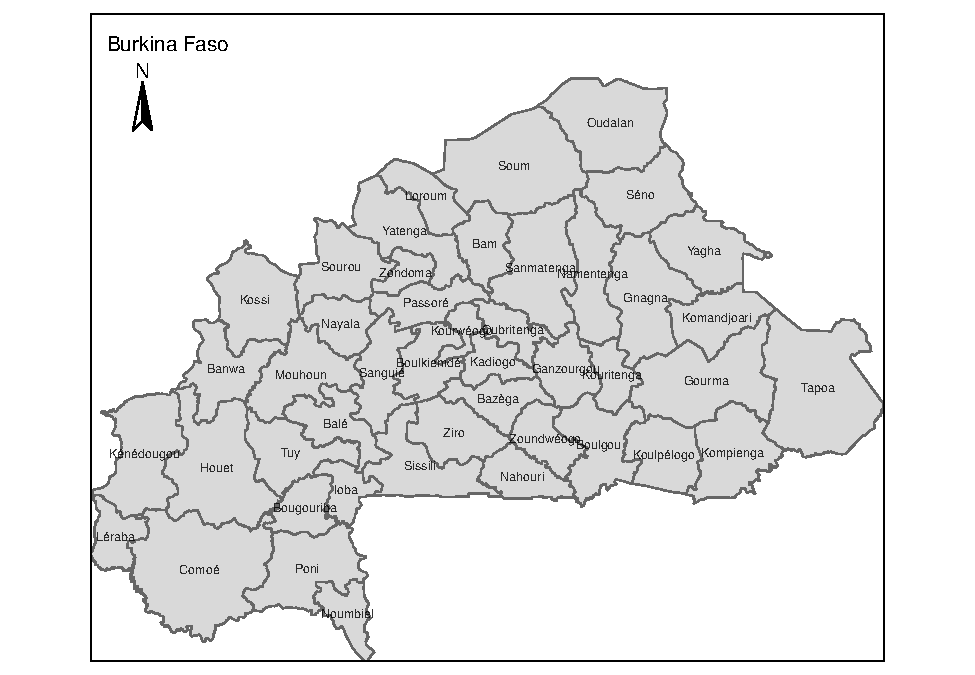
\includegraphics{Document_RMD_GRP_files/figure-latex/spatial-1.pdf}

\subsection{Un peu de statistiques
spatiales(2)}\label{un-peu-de-statistiques-spatiales2}

\begin{Shaded}
\begin{Highlighting}[]
\FunctionTok{library}\NormalTok{(openxlsx)}

\NormalTok{way}\OtherTok{\textless{}{-}} \FunctionTok{paste0}\NormalTok{(past,}\StringTok{"/BKF//température.xlsx"}\NormalTok{)}
\NormalTok{temperature }\OtherTok{\textless{}{-}} \FunctionTok{read.xlsx}\NormalTok{(}\StringTok{"../Document\_Rmarkdown/BKF/température.xlsx"}\NormalTok{)}
\NormalTok{temperature }\OtherTok{\textless{}{-}} \FunctionTok{data.frame}\NormalTok{(temperature)}
\NormalTok{bkf\_2}\OtherTok{\textless{}{-}} \FunctionTok{merge}\NormalTok{(bkf, temperature, }\AttributeTok{by =} \StringTok{"NAME\_2"}\NormalTok{, }\AttributeTok{all.x =} \ConstantTok{TRUE}\NormalTok{)}
\NormalTok{bkf\_2\_T }\OtherTok{\textless{}{-}} \FunctionTok{tm\_shape}\NormalTok{(bkf\_2) }\SpecialCharTok{+} 
  \FunctionTok{tm\_polygons}\NormalTok{(}\StringTok{"Temperature"}\NormalTok{, }\AttributeTok{title =} \StringTok{"Temperature"}\NormalTok{) }\SpecialCharTok{+}
  \FunctionTok{tm\_borders}\NormalTok{(}\StringTok{"white"}\NormalTok{, }\AttributeTok{lwd =} \FloatTok{0.5}\NormalTok{) }\SpecialCharTok{+}
  \FunctionTok{tm\_text}\NormalTok{(}\StringTok{"NAME\_2"}\NormalTok{, }\AttributeTok{size =} \FloatTok{0.5}\NormalTok{, }\AttributeTok{col =} \StringTok{"black"}\NormalTok{, }\AttributeTok{alpha =} \FloatTok{0.8}\NormalTok{)}\SpecialCharTok{+}
  \FunctionTok{tm\_layout}\NormalTok{(}\AttributeTok{title =} \StringTok{"Température du Burkina Faso"}\NormalTok{)}\SpecialCharTok{+}
  \FunctionTok{tm\_compass}\NormalTok{(}\AttributeTok{type =} \StringTok{"arrow"}\NormalTok{, }\AttributeTok{position =} \FunctionTok{c}\NormalTok{(}\StringTok{"left"}\NormalTok{, }\StringTok{"top"}\NormalTok{))}\SpecialCharTok{+}
   \FunctionTok{tm\_scale\_bar}\NormalTok{(}\AttributeTok{position =} \FunctionTok{c}\NormalTok{(}\StringTok{"center"}\NormalTok{,}\StringTok{"bottom"}\NormalTok{))}
\end{Highlighting}
\end{Shaded}

\subsubsection{Résultat}\label{ruxe9sultat-3}

\begin{Shaded}
\begin{Highlighting}[]
\NormalTok{bkf\_2\_T}
\end{Highlighting}
\end{Shaded}

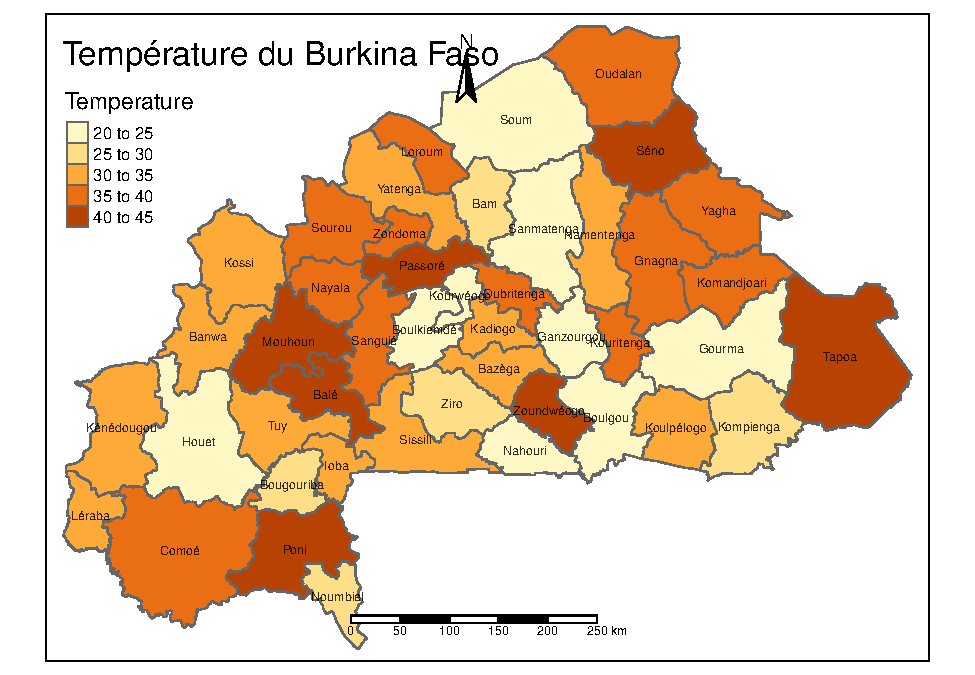
\includegraphics{Document_RMD_GRP_files/figure-latex/plot-1.pdf}

\subsection{Autres fonctionnalités}\label{autres-fonctionnalituxe9s}

Il y a d'autres fonctionnalités de beamer comme : générer la table des
matières, les numéros des sections, les options de sorties,ajouter une
image, les listes etc. Ces fonctionnalités sont discutées plus en détail
dans les présentations générales de Rmarkdown.

\newpage

\section{R Markdown et LateX}\label{r-markdown-et-latex}

Si vous souhaitez concevoir des documents pdf très attrayant, comme
celui-ci d'ailleurs, il est conseillé d'associer vos balises R markdown
aux balises LateX. Nous vous présentons ici quelques balises LateX
simple qui peuvent faire la différence dans vos documents R markdown.
Tous les packages LateX nécessaires doivent être inclus dans l'entête
YAML à l'aide de \texttt{header-includes:} où vous devez lister ces
packages.

\textbf{Les pages de garde :}

Pour insérer une page de garde dans votre document Rmd, vous devez avoir
une page de garde faite à partir de Ms word par exemple. Cette parge de
garde doit être au \textbf{format pdf} et être \textbf{contenu dans le
dossier où se trouve votre script R markdown}.

Avant d'inclure la page de garde, vous devez vous assurer d'inclure le
package LateX qui permet de le faire eu niveau de l'entête YAML. Il
s'agit du package \texttt{\textbackslash{}usepackage\{pdfpages\}}.

La balise permettant d'inclure la page de garde est
\texttt{\textbackslash{}includepdf\{nom\_de\_la\_page\_de\_garde\}}.

\textbf{La table des matières :}

Nous avons déjà vu comment insérer la table de matière avec R markdown,
mais il est conseillé d'utiliser la balise LateX
\texttt{\textbackslash{}tableofcontents} qui permet de générer une table
de matière plus attrayante et qui donne la possibilité de numéroter
automatiquement les parties de notre document.

\textbf{Liste des tableaux et liste des figures :}

Il est aussi possible d'inclure une liste des tableaux et des figures
avec des balises lateX \texttt{\textbackslash{}listoftables} et
\texttt{\textbackslash{}listoffigures}.

\textbf{Insérer une nouvelle page :}

Vous l'aurez remarqué, l'insertion d'une nouvelle page dans R mardown se
fait très souvent à l'aide de la balise lateX
\texttt{\textbackslash{}newpage}.

\textbf{Mettre un texte en couleur :}

Dans vos document R markdown vous pouvez mettre vos titres ou vos textes
en couleur à l'aide de la syntaxe
\texttt{\textbackslash{}textcolor\{nom\_couleur\}\{texte\_ou\_titre\}}.
Par exemple \textcolor{blue}{Le texte suivant s'ecrira en couleur bleu}.

\textbf{Encadrer un texte :}

Pour encadrer votre block de texte, vos pouvez utiliser le block de code
\texttt{\textbackslash{}begin\{tcolorbox\}{[}colframe\ =\ couleur\_du\_block,\ colback\ =\ couleur\_background,\ title\ =\ titre\_du\_paragraphe\ {]}...(votre\ texte)...\textbackslash{}end\{tcolorbox\}}.

Par exemple :

\begin{tcolorbox}[colframe = blue, colback = gray, title = Block de texte ]

Le block de texte suivant nommé 'Block de texte' s'affichera dans un frame de couleur bleue et de fond gris.

\end{tcolorbox}

Vous pouvez aussi utiliser le block de code
\texttt{\textbackslash{}begin\{framed\}...\textbackslash{}end\{framed\}}
du package lateX \texttt{\textbackslash{}usepackage\{framed\}}

Par exemple :

\begin{framed}

Ceci est un bloc de texte encadré.

\end{framed}

\textbf{Alignement de texte :}

Vous pouvez aussi choisir l'alignement de votre texte gauche, droite ou
centré à l'aide des blocks de code lateX
\texttt{\textbackslash{}begin\{flushleft\}...\textbackslash{}end\{flushleft\}},
\texttt{\textbackslash{}begin\{flushright\}...\textbackslash{}end\{flushright\}}
et
\texttt{\textbackslash{}begin\{center\}...\textbackslash{}end\{center\}}.

Exemple :

\begin{center}
Texte centré.
\end{center}

\begin{flushleft}
Texte aligné à gauche.
\end{flushleft}

\begin{flushright}
Texte aligné à droite.
\end{flushright}

\textbf{Labelisation d'equations :}

On peut donner un nom à une equation et la labeliser à l'aide de la
commande LateX \texttt{\textbackslash{}label\{eq:nom\_equation\}}.

\textbf{Exemple :}

\begin{equation}
E = mc^2
\label{eq:emc2}
\end{equation}

On utilise la commande
\texttt{\textbackslash{}eqref\{eq:nom\_equation\}} pour faire apparaître
la référence de l'equation comme ci-dessous.

Comme nous pouvons le voir dans l'équation \eqref{eq:emc2}, l'énergie
est proportionnelle à la masse.

En cliquant sur la référence, on peut revenir voir l'équation.

\textbf{Entête et pieds de pages avec LateX}

Il est possible de ce demander en consultant ce document comment ajouter
les en-têtes et les pieds de pages dans son document R markdown pour les
sorties pdf.

En effet cela nécessite une suite de codes LateX nottament
\texttt{\textbackslash{}renewcommand\{\}},\texttt{\textbackslash{}headrulewidth},\ldots{}

Le code LateX utilisé pour cela est le suivant :

\begin{center}\includegraphics[width=1\linewidth,height=1\textheight]{../Document_Rmarkdown/Images/En-têtes_Pieds_pages} \end{center}

\textbf{NB :}

\textbf{Toutes ces mises en formes ne seront visibles que pour les
sorties sous le format pdf.}

Voici une listes de balises LateX que vous pouvez utiliser pour vos
documents R markdown et leur fonctionnement respectifs.

\begin{figure}

{\centering 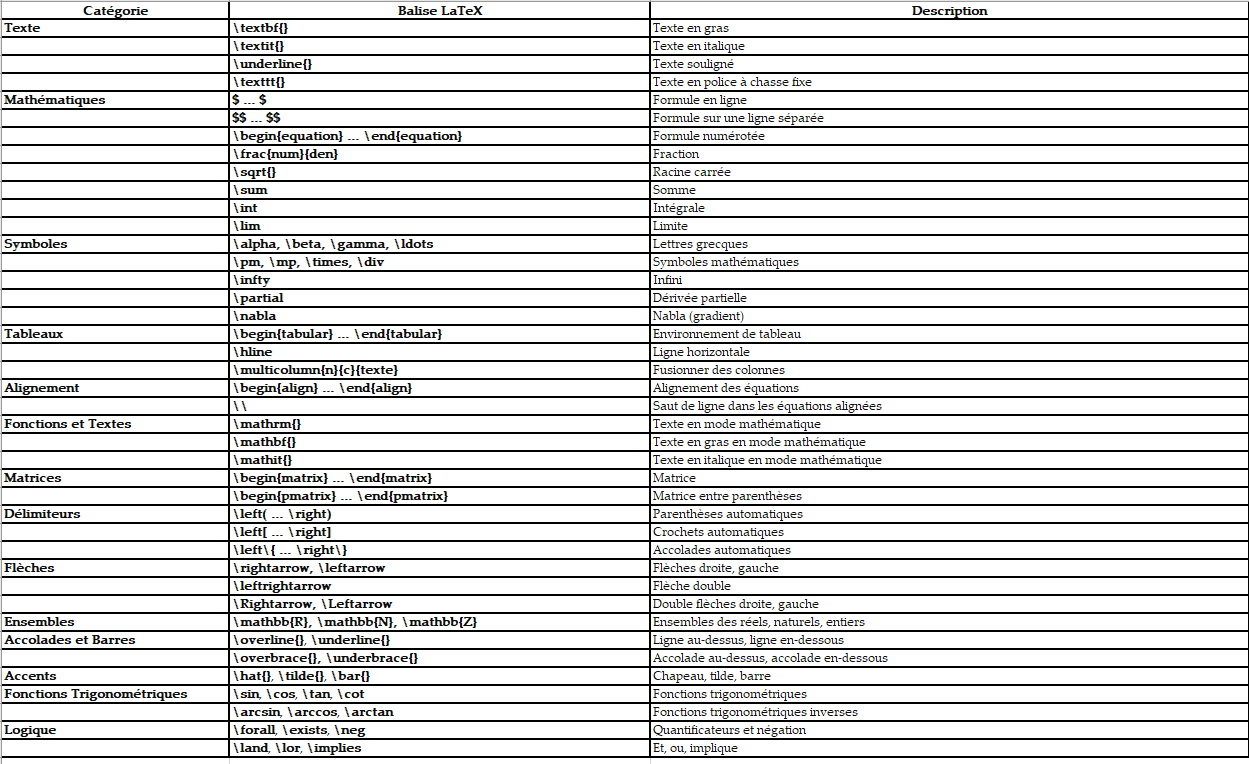
\includegraphics[width=1\linewidth,height=1\textheight]{../Document_Rmarkdown/Images/Balises_LateX} 

}

\caption{Balises LateX}\label{fig:unnamed-chunk-36}
\end{figure}

\newpage

\section{R Markdown, HTML et CSS}\label{r-markdown-html-et-css}

Si vous souhaiter avec des documents interactifs, il est conseillé de
privilégier les sorties HTML qui supportent les graphiques et tableaux
dynamiques, ce qui n'est pas le cas des sorties pdf par exemple.

Vous pouvez utiliser du code CSS pour faire toutes mises en formes de
votre document HTML; vous pourrez même ainsi créer vos propres
templates.

Par exemple, à l'aide du code CSS suivant :

\begin{center}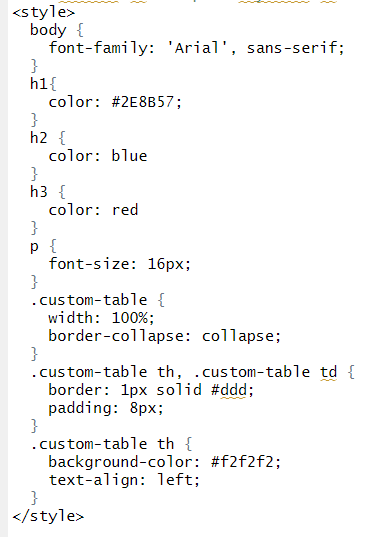
\includegraphics[width=0.5\linewidth,height=0.5\textheight]{../Document_Rmarkdown/code_CSS} \end{center}

On obtient la sortie HTML suivante :

\begin{center}
\includegraphics[width=1\linewidth,height=1\textheight]{../Document_Rmarkdown/Sortie_code_CSS} \end{center}

\textbf{NB :} Les graphiques et tableaux dynamiques ne sont pas
supportés sous le format pdf. Si vous effectuez une telle sortie R vous
renverra des erreurs. Pour corriger ceux-ci, vous devez ajouter l'option
\textbf{\texttt{always\_allow\_html:\ true}} dans l'entête YAML.

\newpage

\section{Creation de livre avec bookdown de R
markdown}\label{creation-de-livre-avec-bookdown-de-r-markdown}

Pour la création de livre avec R markdown, rassurez-vous tout d'abord
d'installer le package \texttt{bookdown} avec par exemple la commande
\texttt{install.packages("bookdown")}.

Ensuite suivez les étapes suivantes :

\begin{enumerate}
\def\labelenumi{\arabic{enumi}.}
\item
  Allez dans \texttt{File} -\textgreater{} \texttt{New\ Project}.
\item
  Sélectionnez \texttt{New\ Directory}.
\end{enumerate}

\begin{center}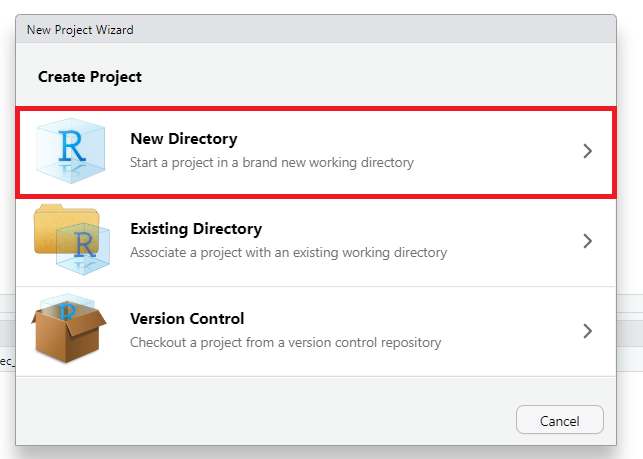
\includegraphics[width=0.7\linewidth,height=0.7\textheight]{../Document_Rmarkdown/Images_creation_livres/New_directory} \end{center}

\begin{enumerate}
\def\labelenumi{\arabic{enumi}.}
\setcounter{enumi}{2}
\tightlist
\item
  Choisissez \texttt{Book\ Project\ using\ bookdown}.
\end{enumerate}

\begin{center}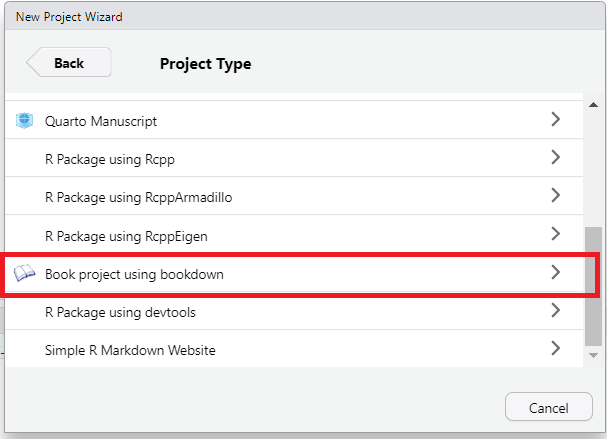
\includegraphics[width=0.7\linewidth,height=0.7\textheight]{../Document_Rmarkdown/Images_creation_livres/book_using_bookdown} \end{center}

\begin{enumerate}
\def\labelenumi{\arabic{enumi}.}
\setcounter{enumi}{3}
\tightlist
\item
  Donnez un nom à votre projet et sélectionnez un dossier pour le
  sauvegarder et Cliquez sur \texttt{Create\ Project}.
\end{enumerate}

\begin{center}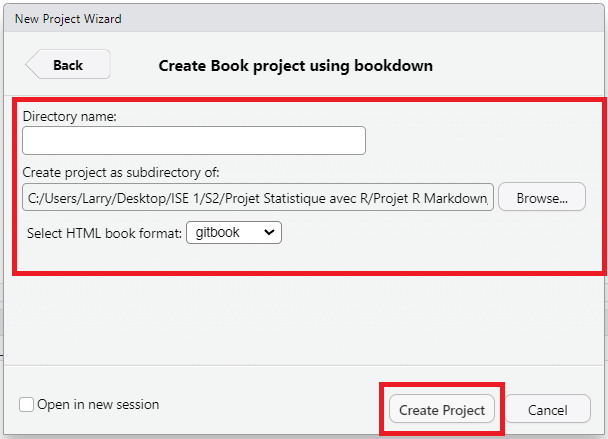
\includegraphics[width=0.7\linewidth,height=0.7\textheight]{../Document_Rmarkdown/Images_creation_livres/Create_projet} \end{center}

Une structure de répertoire sera générée par défaut pour votre livre.

\begin{center}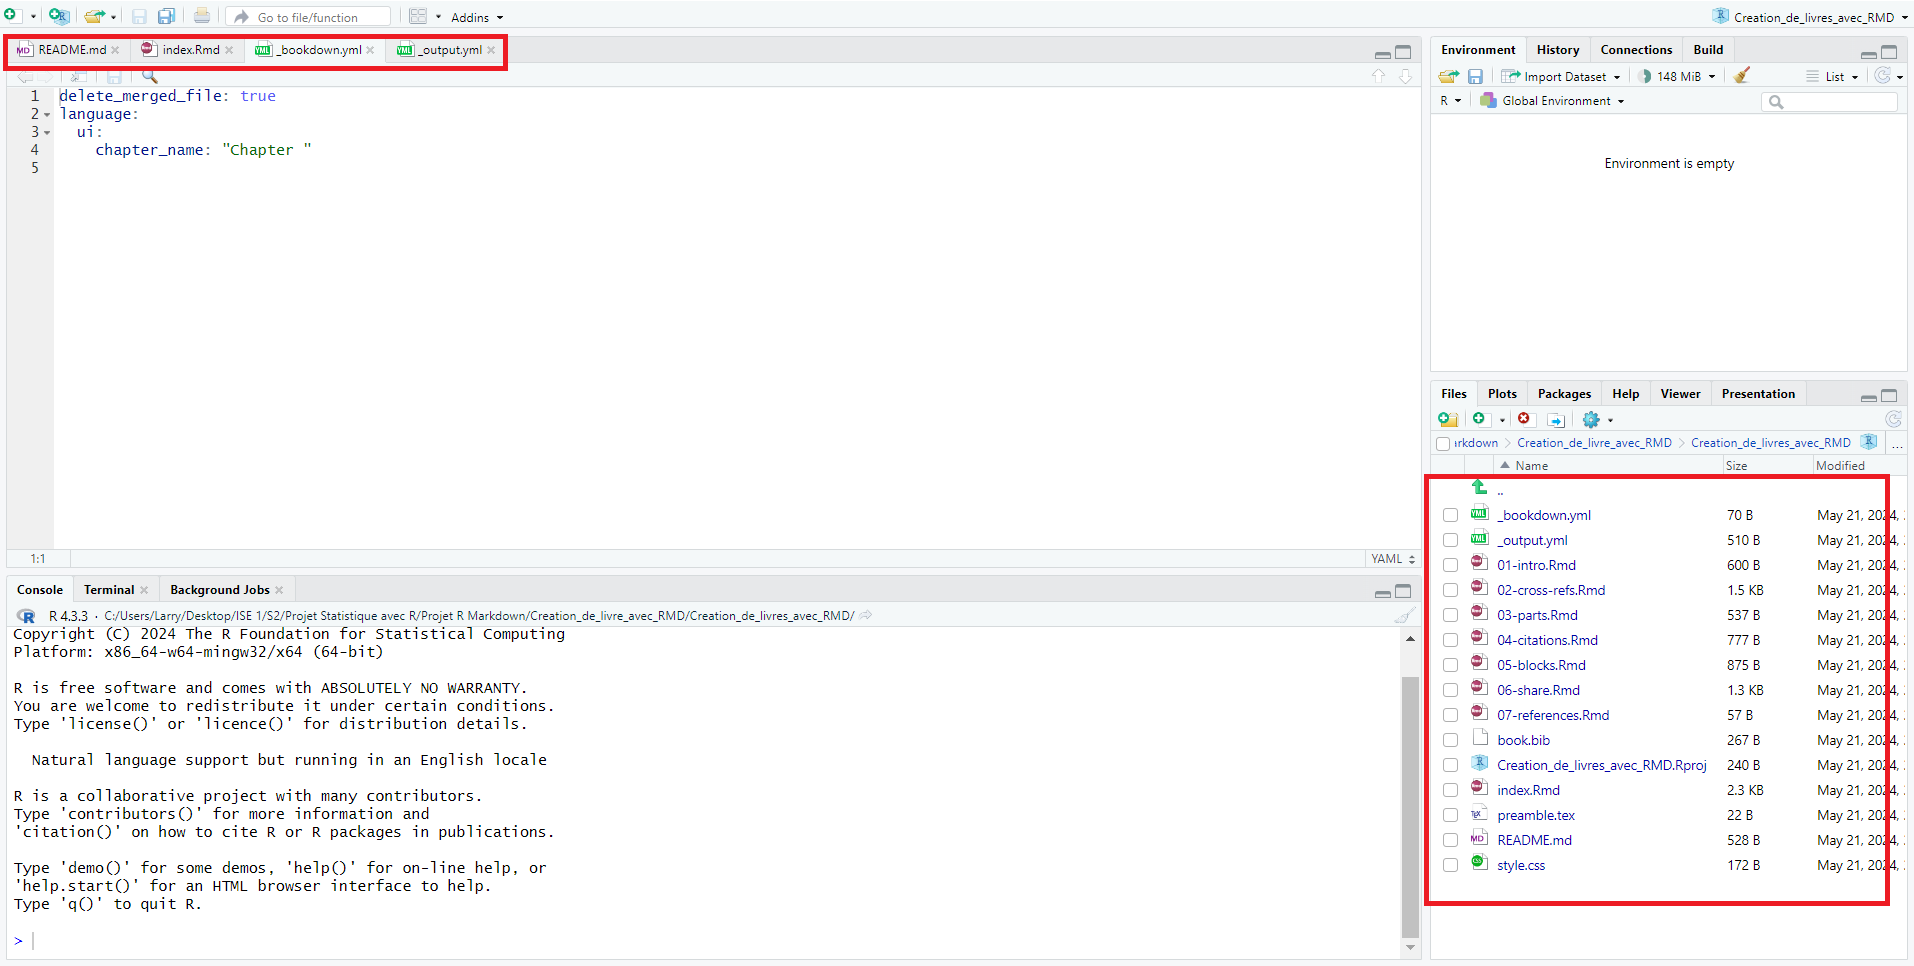
\includegraphics[width=1\linewidth,height=1\textheight]{../Document_Rmarkdown/Images_creation_livres/Affichage_Projet} \end{center}

La structure de base générée inclut les fichiers suivants :

\begin{itemize}
\tightlist
\item
  \texttt{\_bookdown.yml} : Fichier de configuration pour Bookdown.
\item
  \texttt{index.Rmd} : Page de titre et de préface de votre livre.
\item
  \texttt{01-intro.Rmd}, \texttt{02-chap.Rmd}, etc. : Chapitres de votre
  livre.
\item
  \texttt{book.bib} : Fichier de références bibliographiques (si
  nécessaire).
\item
  \texttt{output.yml} : Configuration des formats de sortie (PDF, HTML,
  ePub).
\end{itemize}

Vous pouvez ensuite configure le \texttt{\_bookdown.yml} de façon à
organiser votre livre comme vous le souhaitez.

\hyperref[Introduction]{retour à introduction}

\textbf{Compilation du livre}

Pour compiler le livre, vous pouvez utiliser :

\begin{itemize}
\item
  \textbf{\texttt{bookdown::render\_book("index.Rmd",\ "bookdown::pdf\_book")}}
  pour compiler en \textbf{pdf}
\item
  \textbf{\texttt{bookdown::render\_book("index.Rmd",\ "bookdown::epub\_book")}}
  pour compiler en \textbf{epub}
\end{itemize}


\includepdf{Fin_Page_de_garde.pdf}

\end{document}
